\documentclass[10pt,a4paper,twoside,titlepage,twocolumn]{article}
\usepackage[utf8]{inputenc}
\usepackage[T1]{fontenc}
\usepackage[ngerman]{babel,varioref}
\usepackage[left=0.7cm,right=0.7cm,top=0.7cm,bottom=0.7cm,includeheadfoot]{geometry}

\usepackage{amsmath}
\usepackage{amssymb}
\usepackage{graphicx}
\usepackage{xcolor}
\usepackage{siunitx}
\usepackage{enumitem}
\usepackage{transparent}



\begin{document}
    \graphicspath{ {./Images/} }


\definecolor{formulablue}{RGB}{219,219,255}
\newcommand{\formula}[1]{\colorbox{formulablue}{#1}}

\newcommand{\unitText}[3]{\noindent\textit{#1} : #2 [#3]}

\definecolor{refrot}{RGB}{183,28,42}
\newcommand{\refskript}[1]{\textcolor{refrot}{Skript S.#1}}



% \titlespacing*{\section}{0pt}{12pt}{0pt}
% \titlespacing*{\subsection}{0pt}{0pt}{0pt}
% \titlespacing*{\subsubsection}{0pt}{0pt}{0pt}


\title{\vspace{50mm}MachLe \\ [1ex] \large Summary}
\author{Lukas Schöpf}
% \titlepic{\vspace{50mm}\includegraphics[width=0.25\textwidth]{Elvis}}


% Code format
% Define the Gruvbox light colors
\definecolor{gruvbox_bg}{HTML}{fbf1c7}
\definecolor{gruvbox_fg}{HTML}{3c3836}
\definecolor{gruvbox_yellow}{HTML}{d79921}
\definecolor{gruvbox_red}{HTML}{cc241d}
\definecolor{gruvbox_green}{HTML}{98971a}
\definecolor{gruvbox_blue}{HTML}{458588}
\definecolor{gruvbox_purple}{HTML}{b16286}
\definecolor{gruvbox_aqua}{HTML}{689d6a}
\definecolor{gruvbox_orange}{HTML}{d65d0e}


% \lstdefinestyle{cppstyle}{
% 	language=C++,
% 	basicstyle=\ttfamily\footnotesize,
% 	numbers=left,
% 	numberstyle=\tiny,
% 	numbersep=5pt,
% 	tabsize=4,
% 	showspaces=false,
% 	showstringspaces=false,
% 	frame=single,
% 	rulecolor=\color{gruvbox_fg},
% 	backgroundcolor=\color{white},
% 	keywordstyle=\color{gruvbox_orange},
% 	commentstyle=\color{gruvbox_aqua},
% 	stringstyle=\color{gruvbox_green},
% 	identifierstyle=\color{gruvbox_fg},
% 	emphstyle=\color{gruvbox_red},
% 	emph={int, double, string, cout, TimerHandle_t, BaseType_t, timerPWMPeripheral_t, SemaphoreHandle_t, TaskHandle_t, QueueHandle_t},
% 	xleftmargin=5mm,
% 	xrightmargin=\parindent
% }

	\maketitle
	\setlength\parindent{0pt}

	% Uncomment these lines if you want to include the respective sections
	\section{Introduction}
\subsection{Data Types}
\begin{itemize}
    \item Numerical/Quantitive, discret: Countable
    
    Example: Number of rejected Loans, classes taken this semster
    \item Numerical/Quantitive, Continuos: Interval data 
    
    Example: Distance, mg of drug taken, size of a house
    \item Categorical, ordinal: distinct and can be ordered
    
    Example: Credit score can be \{low, medium, high\}
    \item Categorical, nominal: categories cannot be orderd
    
    Example: gender, eye color
\end{itemize}
\subsection{Machine Learning Paradigms}
\begin{itemize}
    \item Unsupervised Learning: Discover and explore structure from unlabelled data
    \item Supervised Learning: Learn to predict/forecast an output of interest, we know what we want to predict and labelled data is available
\end{itemize}
\subsubsection{Unsupervised Learning}
Tasks:
\begin{itemize}
    \item Dimensionality reduction
    \item Feature Learning
    \item Matrix compilation
    \item Anomaly detection
    \item Generating data
\end{itemize}

 \subsubsection{Supervised Learning}
 Given a set of features/attributes for some objects and also the ouput/target value of what we want to predict.
 The Supervised ML task: Given a new object and its features what would be the output value:
 \begin{itemize}
    \item Regression: Ouput is a numeric value
    \item Classification: Ouput is a categorical value
 \end{itemize}

 \subsection{Data Preparation/Preprocessing}
 Data will rarly be in the format and quality needed for analytics and model training and several of these operations will be needed:
 \begin{itemize}
    \item Data integration/consolidation: Collects and merges data from multiple sources into coherent data store 
    \item Data cleaning: removing or modifying incorrect data, identify and reduce noise in data
    \item Data transformations: normalize, discretize or aggregate the data
    \item Data reduction: reduce data size by reducing the number of samples or reducing the number of attributes, balance skewed data
 \end{itemize}
 Low quality data will result in low quality results


	\section{Supervised ML, Similarities, kNN \& Performance measurments}

\subsection{Supervised ML}
\begin{itemize}
    \item Goal: Find the best Hypothesis
    \[
    H^* = \arg \min_{H\in\mathcal{H}}\sum_{i=1}^{n}loss(x_i,y_i)
    \]
    \item Loss: 
    \[
        loss(x_i,y_i) = (H(x_i) - y_i)^2
    \]
    \item Model: \(H(x) = a + bx + cx^2 + \cdot\)
\end{itemize}
Task of the Learning Algorithem to find best parameters \(a,b,c\)(those that minimize the loss)
\subsubsection{Overfitting}
Model learns traning data but doesnt generalize well.

\subsubsection{Training and test error}
Dataset gets split in Training set and Test set (80\%/20\%)
\(error_{train}\): Error form trained model on train set

\(error_{test}\): Estimate of the true error (generalization error). Error from trained model on test set.
\subsection{kNN}
Pros:
\begin{itemize}
    \item Simple and intuitive
    \item Multiclass
    \item Interpretable 
\end{itemize}
Cons:
\begin{itemize}
    \item Curse of Dimensionality
    \item Sensitive to noise
    \item Computationally expensive for large datasets
\end{itemize}
Given training set \(X = (x_1,\text{class}_1)(x_2,\text{class}_2)\)

Given a new instance \(x_?\):
\begin{itemize}
    \item Find the k-closest examples \(x_i\) to \(x_?\) in the traning set
    \item Classify \(x_?\) based on the majority vote of \(\left\{x_{NN1},x_{NN2},\dots\right\}\)
\end{itemize}
\subsubsection{Distance and similarity measurments}
\begin{figure}[!h]
    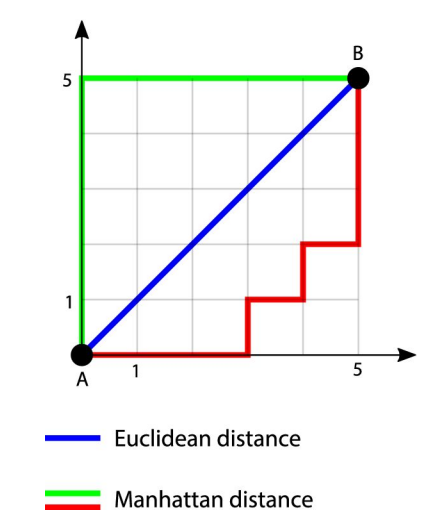
\includegraphics[width = 0.4\columnwidth]{figures/02/distances.png}
\end{figure}
Given 2 point \(\mathbf{q} = (q_1,q_2,\dots,q_n)\) and \(\mathbf{p}= (p_1,p_2,\dots,p_n)\).
\(n\) is the number of dimensions.
\subsubsection*{Euclidean Distance}
\[
d(\mathbf{q},\mathbf{p}) = \sqrt{\sum_{i=1}^{n}(q_i- p_i)}
\]
\subsubsection*{Manhatten Distance}
\[
    d(\mathbf{q},\mathbf{p}) = ||\mathbf{q}-\mathbf{p}||_1 = \sum_{i= 1}^{n}|q_i-p_i|
\]

\subsection{Finding k}
\(k_{opt} \in \{1,2,\dots,N\}\) N = \# of training samples

Extreme cases:
\begin{itemize}
    \item \(k = 1\): kNN = NN
    \item \(k = N\): Majority class
\end{itemize}
\subsection{Performance measures}
\begin{itemize}
    \item Accuracy: \#corr / \#all = (TP + TN) / (TP + FN + FP + TN)
    \item Error: \#wrong / \#all = 1 -  Accuracy
    \item Recall,Sensitivity: TP /(TP + FN), How many relevant samples are correctly detected
    
    \item Specificity: TN/(TN + FP)
    \item Precision: TP/(TP + FP), How many detected samples are relevant
    \item F1 score: 2 \(\cdot\) Precision \(\cdot\) Recall / ( Precision + Recall)
\end{itemize}

\subsubsection{ROC (Receiver Operating Characteristic) curve}
TPR, FPR, to find best threshold.
\begin{figure}[!h]
    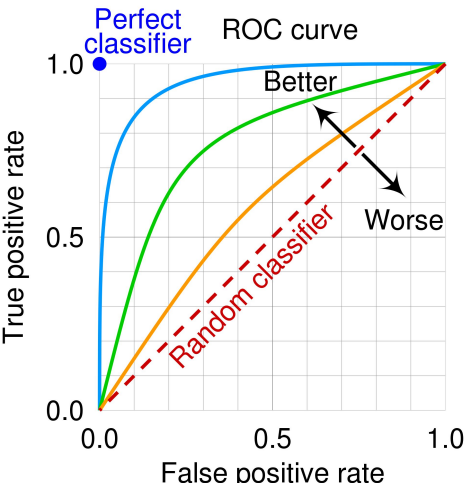
\includegraphics[width = 0.45\columnwidth]{figures/02/ROC.png}
    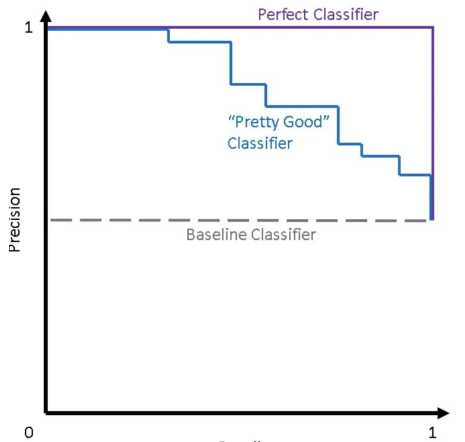
\includegraphics[width =0.45 \columnwidth]{figures/02/PRC.png}
\end{figure}

\subsubsection{PRC(Precision-Recall Curve)}
Precision, Recall, to find best threshold.


	\section{Bias-Varinace tradeoff}
\begin{figure}[!h]
    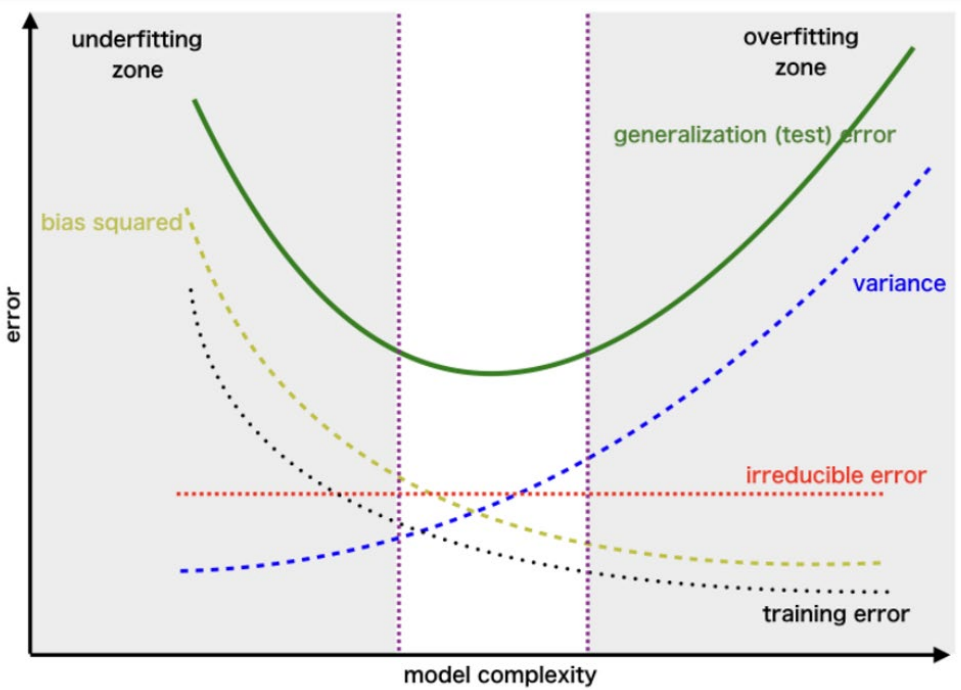
\includegraphics[width = \columnwidth]{figures/03/BiasVariance.png}
\end{figure}
\subsection{No free lunch Theorem}
There is no universally best learner (across problems):

\subsection{Ockham's Razor}
Given 2 models with the same empirical (test) error, the simpler one should be preferred because simplicity is desirable in itself.
\subsection{Error sources and bias-variance tradeoff}
Different Error sources:
\begin{itemize}
    \item The model: the best hypothesis is at distance to the true function
    \item The dataset: different datasets potentially provide different information
    \item Uncertainty in (X,Y) and its representation:
    \subitem Partial view of the task: have all relevant features been observed?
    \subitem Noisy data
\end{itemize}

Error Decomposit MSE:
\[
E_{MSE} = bias + variance + Irreducible \,error
\]
Bias(systematic error): average predictions deviation from the truth

Variance(dependence on specific sample): Sensitivity of prediction to specific training sample

Irreducible error(random nature of process): due to noise

Generally, for more complex/capable model: bias \(\downarrow\),variance \(\uparrow\). Its a trade-off: Only way to redue both is to increase the size of the dataset.

\subsection{Model selection: Validation score and CV score}
\begin{figure}
    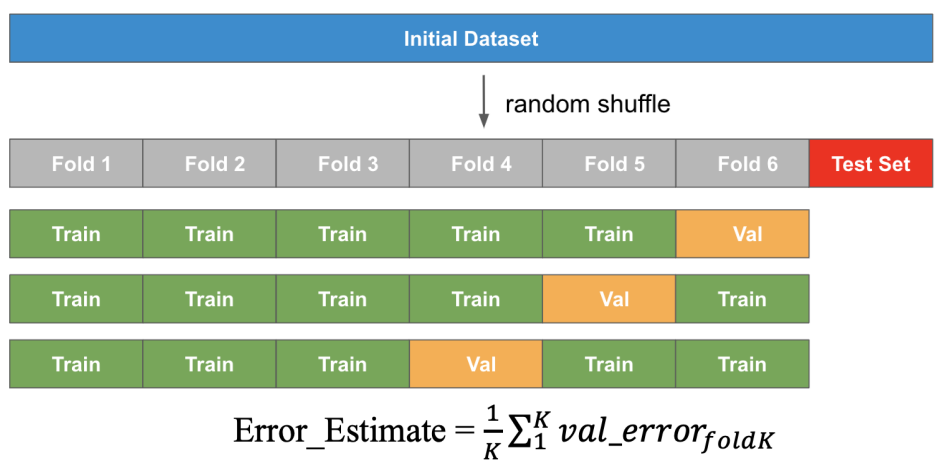
\includegraphics[width = \columnwidth]{figures/03/CV.png}
\end{figure}
k-Fold Corss Validation(CV): We can get a more realistic estimate of the test error using many validation sets (Typically K is 5 to 10)

\subsubsection{Error Estimate Summary}
In practice:
\begin{itemize}
    \item Validation score(s) or CV score provide estimates of the test error
    \item The test error provides an estimate of the true error
    \item Never use any test data in the model training and model selection process
\end{itemize}
Which model to choose?
\begin{itemize}
    \item The one with best validation or CV score
    \item Use student's t-test to check that an improvement is significant
    \item Ockham's razor: prefer simpler models in abscence of other evidence
\end{itemize}
Model selection is an empirical science.
\subsection{Loss minimization (gradient descent)}
Linear Model: \(f(x) = w_0 + w_1 x = \hat{y}\)
\[
RSS = \sum_{i = 1}^{N} (y_i - \hat{y_i})^2
\]
Use gradient of RSS to find optimal weights for model.
\[
\mathbf{w}_{new} = \mathbf{w}_{old}- stepsize \cdot \frac{df(\mathbf{w})}{d\mathbf{w}}
\]
The effectiveness of gradient descent depends on the choice of the learning rate (step size):
\begin{itemize}
    \item Too big, might not reach optimal value
    \item Too small, it will take a long time to converge
\end{itemize}
\subsection{Regularization}
\begin{figure}[!h]
    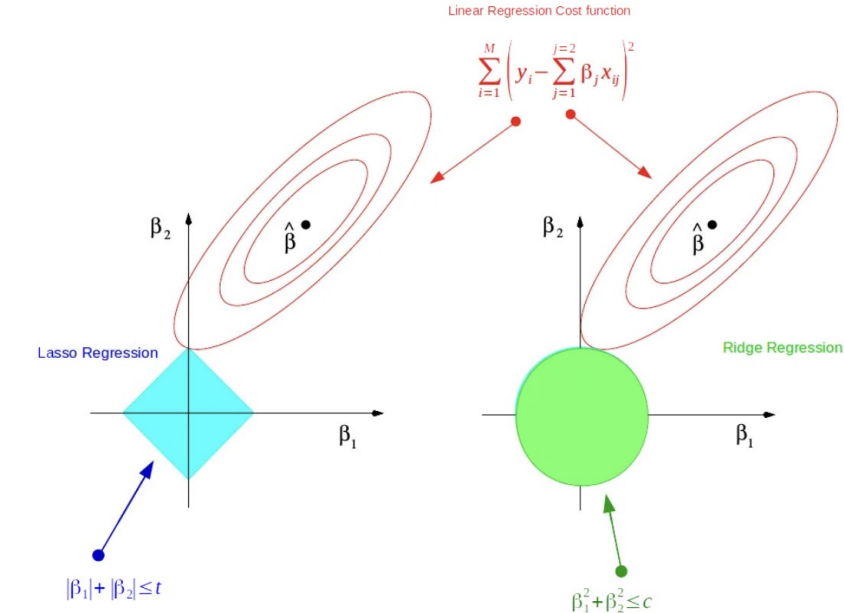
\includegraphics[width = \columnwidth]{figures/03/Regression.png}
\end{figure}

Reduce overfitting of model by penalizing model complexity

Tradeoff:
\begin{itemize}
    \item increase bias
    \item decrease variance
\end{itemize}
\[
H^* = \arg\min_{H \in \mathcal{H}}\sum_{i = 1}^{n}\mathcal{L}_\theta(x_i,y_i) + \lambda R(H)
\]
\(R(H)\) is the models complexity.
\(\lambda\) controlls the model complexity.
\begin{itemize}
    \item Lasso:\(\text{L}_1\) regularization
    \[
    \arg\min\underbrace{||y-X\beta||_2^2}_{\text{Loss}} + \lambda\underbrace{||\beta||_2^2}_{\text{Penalty}}
    \]
    \item Ridge:\(\text{L}_2\) regularization
    \[
    \arg\min\underbrace{||y-X\beta||_2^2}_{\text{Loss}} + \lambda\underbrace{||\beta||_1}_{\text{Penalty}}
    \]
\end{itemize}

\subsection{Hyperparameter tuning}
\begin{figure}[!h]
    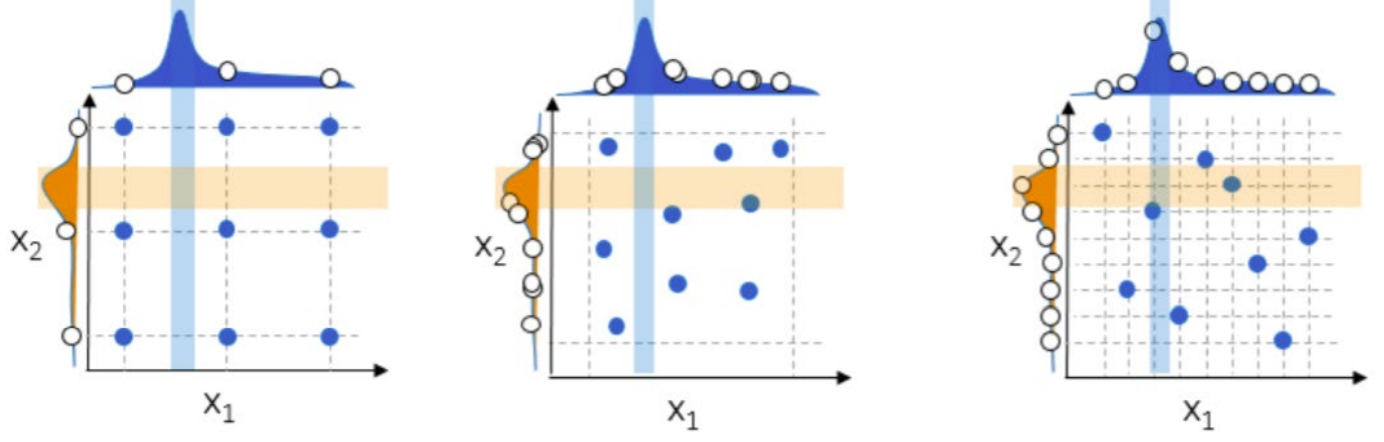
\includegraphics[width = \columnwidth]{figures/03/Hyperparameter.png}
\end{figure}
\begin{itemize}
    \item Grid-search
    \item Random-search
    \item \{Optimization\}
\end{itemize}
	\section{Decision Tree, Ensamble Methods \& Random Forest}
\subsection{Decision Tree}
\begin{itemize}
    \item A flow-chart-like tree structure
    \item Internal node denotes a test on a attribute
    \item Branch represent an outcome of the test
    \item Leaf nodes represent class labels or class distribution
\end{itemize}
Gini Index:
\[
I_G = 1- \sum_{j = 1}^{c}p_j^2
\]
Entropy:
\[
I_H = - \sum_{j = 1}^{c} p_j \log(p_j)
\]
\(p_j\) is the proportion of samples that belongs to calss \(j\).
Tree construction:
\begin{enumerate}
    \item Initialization: whole region \(R_0\)(i.e., all given data)
    \item Repeat:
    \begin{itemize} 
        \item For each region \(R_i\), for each feature \(X_j\), for each split \(R_i = R_{i,l} \cup R_{i,r}\) with respect to feature \(x_j\). Calculate change in impurity score (e.g., gini, entropy, error)
        \item Choose best split,i.e., maximum decrease of the impurity score
        \item Replace \(R_i\) with the two new split regions
    \end{itemize}
\end{enumerate}
Avoiding overfitting:
\begin{itemize}
    \item Select a proper depth of the tree
    \item Select a proper minimum number of samples in a leaf to stop further splitting
    \item Tree pruning - remove split nodes bottom up or top down
\end{itemize}
All these performed using either a validation set or cross validation!

\subsection{Pros/Cons}
Pros:
\begin{itemize}
    \item Easily visualized and interpreted
    \item No feature normalization or scaling needed
    \item Works well with mixed feature data types (categorical, continuous)
\end{itemize}
Cons:
\begin{itemize}
    \item Easly ovefits
    \item Not robust, high variance
\end{itemize}
\subsection{Ensamble methods}
Appproach:
\begin{itemize}
    \item Suppose you have \(n\) classifier
    \item Each classifier has error rate \(e\) 
    \item Assume the classifier are independent
    \item Take Majority vote
\end{itemize}
The combined result is wrong if \(n/2\) classifiers are wrong.
According  to central limit theorem variance reduces by factor \(n\).
\subsubsection{Bagging}
\begin{figure}[!h]
    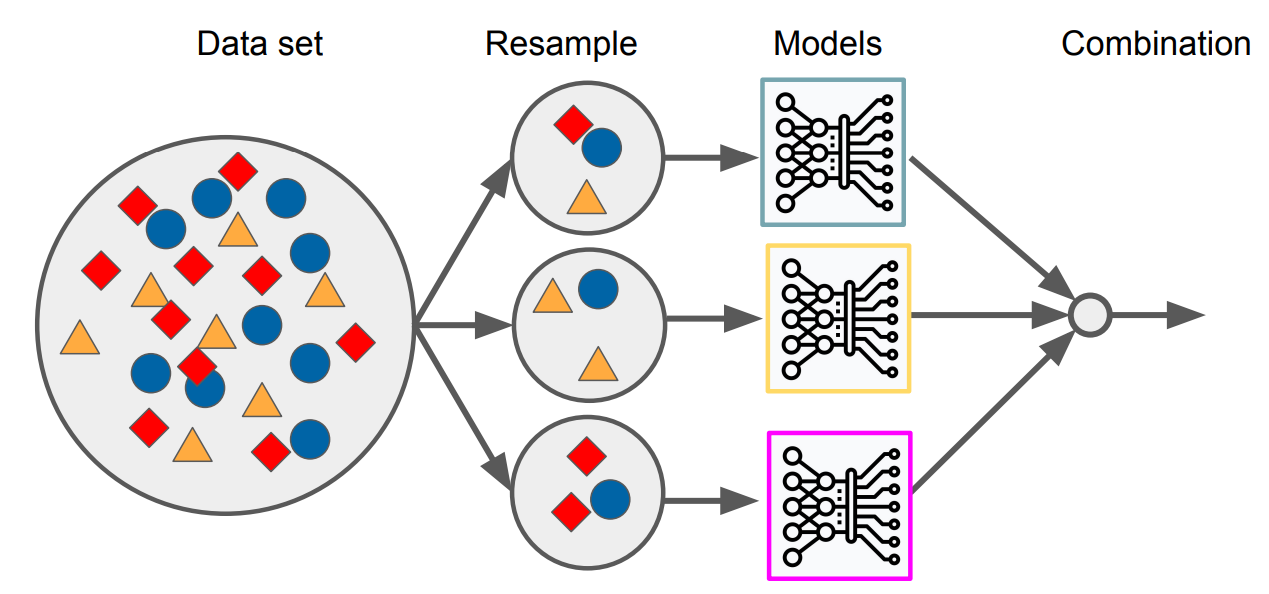
\includegraphics[width = \columnwidth]{figures/04/Bagging.png}
\end{figure}
To have independent classifier use many independent training sets \(S_i\) to train models.
\begin{itemize}
    \item Variance reduces linearly (sub-linearly in practice beacuse \(S_i\) are correlated)
    \item Bias unchanged (increases slightly in practice)
\end{itemize}

\subsubsection{Boosting}
Weight samples. Samples where the model makes mistakes are weighted higher.

Algorithm:
\begin{enumerate}
    \item Initialization: Train first model on data
    \item Repeat:
    \begin{itemize}
        \item Compute error of the model on each training sample
        \item Give higher importance to samples where the model makes mistakes
        \item Train next model using importance weighted training samples
    \end{itemize}
\end{enumerate}
In each iteration, introduce a weak model to compensate the shortcoming of the existing string (= combined) model.
\subsubsection*{Adaptive Boosting(AdaBoost)}
Take a weak learning algorithm and turn it into a strong one by making it focus more on the accurate predictions of difficult cases.
\[
F_T(x) = \sum_{t = 1}^{T}f_t(x)
\]
In each iteration \(t\):
\begin{itemize}
    \item A new weak classifier \(h(x_i)\) with a coefficant \(\alpha\) is added to the existing ones such that the error \(E_t\) of the ensemble at iteration \(t\) is minimized.
    \[
    E_t = \sum_{i}\left[F_{t-1}(x_i) + \alpha_t h(x_i)\right]
    \]
    \item The new weak classifier is training using a weighted training set where the weight assigned to each sample is identical to the error of the current ensemble classifier on that sample \(E(F_{t-1}(x_i))\).
\end{itemize}
\subsubsection{Comparison}
No Ensamble:
\begin{itemize}
    \item complete training set, train one model
\end{itemize}
Bagging:
\begin{itemize}
    \item randomly sample with replacement to obtain different training set
    \item minimizes variance (usually cannot reduce bias) -- fights overfitting
    \item Computationally efficient (all models can be trained in parallel)
\end{itemize}
Boosting:
\begin{itemize}
    \item randomly sample with replacement over weighted data to obtain different trainin sets
    \item Minimize bias by adding models to the ensemble -- fight underfitting
    \item Address variance by using simple models with low variance
\end{itemize}
\subsubsection{Random forest}
\begin{figure}[!h]
    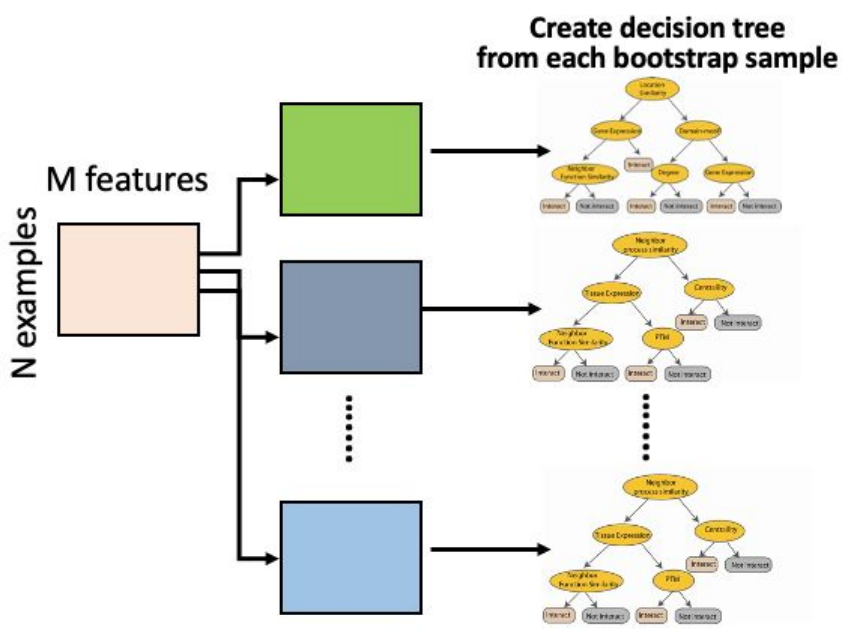
\includegraphics[width =\columnwidth]{figures/04/RandomForrest.png}
\end{figure}
Basic idea:
\begin{itemize}
    \item Grow many trees in bootstrapped samples of training data
    \item Minimize bias by growing trees sufficiently deep (overfitting)
    \item Maximize variance reduction by minimizing correlation between trees by means of bootstrapping data for each tree and sampling variable set at each node
    \item Reduce variance of noisy but unbiased trees by averaging
\end{itemize}
\subsubsection*{Out of Bag Errors (OOB Error)}
\begin{figure}[!h]
    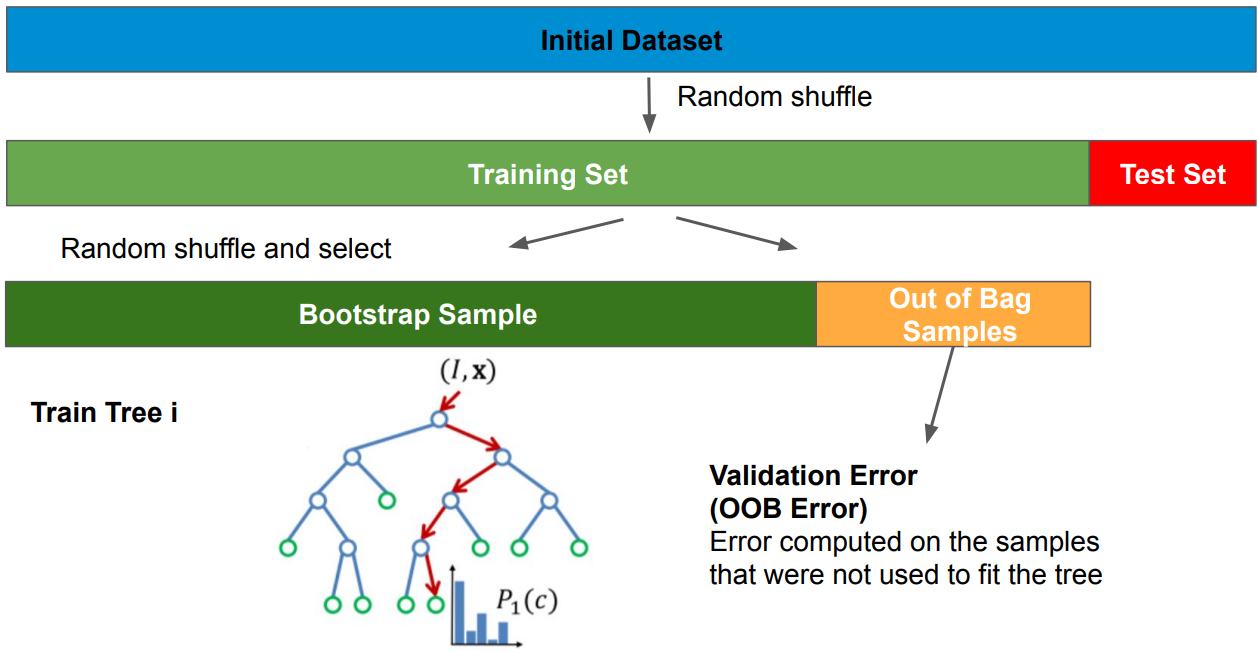
\includegraphics[width = \columnwidth]{figures/04/OOBError.png}
\end{figure}
\subsubsection{Summary Random Forrest}
Pros:
\begin{itemize}
    \item Simple - no assumption of the underlying distribution
    \item OOB error for free
    \item Many variables, even when they are not relevant for the task at hand or noisy
    \item Robust against outliers
    \item Multiclass
    \item Limit overfitting (trees have to be independent!)
    \item Unbalanced dataset (supsampling)
\end{itemize}
	\section{Probability Recap, Loss Functions, Logistic Regression, Neural Networks Intro}
\subsection{Probability Basics}
\textbf{Random Variable (RV)} \(x\) denotes a quatity that is uncertain, discret or continuous.
\(p(x = \mathbb{X})\): the probability of variable \(x\) being in state \(\mathbb{X}\).

\textbf{Domain of RV} denotes all the values it can take (states it can be in).
\(\text{dom}(coin) = \{\text{heads,tails}\}\)


\textbf{Joint distribution} of two RVs \(x\) and \(y\) takes a particular combination of values and the joint probability density satisfies:
\[
\int\int Pr(x,y) \cdot dxdy = 1
\]

\textbf{Marginal distributions} \(Pr(x)\) and \(Pr(y)\) are obtained by:
\[
    \int\ Pr(x,y) \cdot dx = Pr(y)
\]
\[
    \int\ Pr(x,y) \cdot dy = Pr(x)
\]

Conditional probability \(Pr(x|y)\) is the probability of a variable \(x\) taking a certain value assuming we know the value of \(y\):
\[
Pr(x|y) = \frac{Pr(x,y)}{Pr(y)}
\]

\subsubsection{probability rules}
Sum rule:
\[
p(X) = \sum_{Y}p(X,Y)
\]
Product rule:
\[
p(X,Y) = p(Y|X) \cdot p(X) = p(X|Y) \cdot p(Y)
\]
Bayes Theorem:
\[
p(Y|X) = \frac{p(X|Y)\cdot p(Y)}{p(X)} = \frac{p(X|Y)\cdot p(Y)}{\sum_{y \in Y}p(X,y)} = \frac{p(X|Y)\cdot p(Y)}{\sum_{y}p(X,y)\cdot p(y)}
\]
\subsubsection*{Probability distributions and PDFs}
\[
\mathbb{E}\left[x\right] = \mathbb{E}_{x \sim p}\left[x\right] = \int x \cdot p(x)\,dx = \mu
\]
\[
\mathbb{E}\left[x^2\right] = \mathbb{E}_{x \sim p}\left[x^2\right] = \int x^2 \cdot p(x)\,dx = \mu^2 + \sigma^2
\]
\[
\mathbf{VAR}\left[x\right] = \mathbb{E}\left[x^2\right] - \mathbb{E}\left[x\right] = \sigma^2
\]
\subsection{Designing Loss Functions}
Loss/cost function measures how bad the model is - the lower the value of the loss function the better the model maps inputs to output \(\hat{\phi} = \arg\min\left[\text{L}[\phi]\right]\).

Model training is finding parameter values that minimize the loss.

The negative log likelihood (to be minimized) gives us a loss function.
\[
\hat{\phi} = \arg\min_\phi\left[-\sum_{i = 1}^{I}\log\left[Pr(y_i|f(x_i,\phi))\right]\right]
\]
\subsection{Logistic Regression}
Binary classification.
Output is the probability that the input belongs to a class.
\[
y = \text{logistic}(\mathbf{w}^T\mathbf{x}) = \frac{1}{1 + e^{-\mathbf{w}^T\mathbf{x}}}
\]
\subsubsection{Loss function (Binary Cross Entropy Loss)}
\[
J(\theta) = -\frac{1}{N}\sum_{i = 1}^{N}\left[y_i \log\hat{y_i}+  (1-y_i)\log(1-\hat{y_i})\right]
\]
Leads to the following update rule:
\[
\theta_j = \theta_j - \alpha\frac{\partial J(\theta)}{\partial \theta_j}
\]
this is simplified to:
\[
    \theta_j = \theta_j - \alpha\frac{1}{N}\sum_{i = 1}^{N}(\hat{y_i}-y_i)x^{(j)}_i
\]

\subsection{Neural Networks Basics}
Neural Networks (NN) consist of Neurons.
The value of a Neuron is defined by its connections to tha last layer, the weights(\(w_i\)) of the connection, the bias(\(b\)) and the activation funtion of the Neuron.
\begin{figure}[!h]
    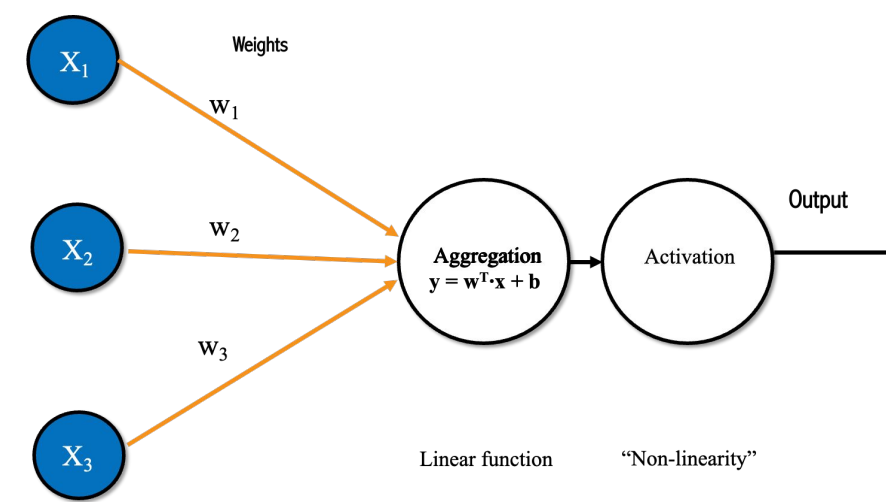
\includegraphics[width = \columnwidth]{figures/05/Neuron.png}
\end{figure}
\begin{figure}[!h]
    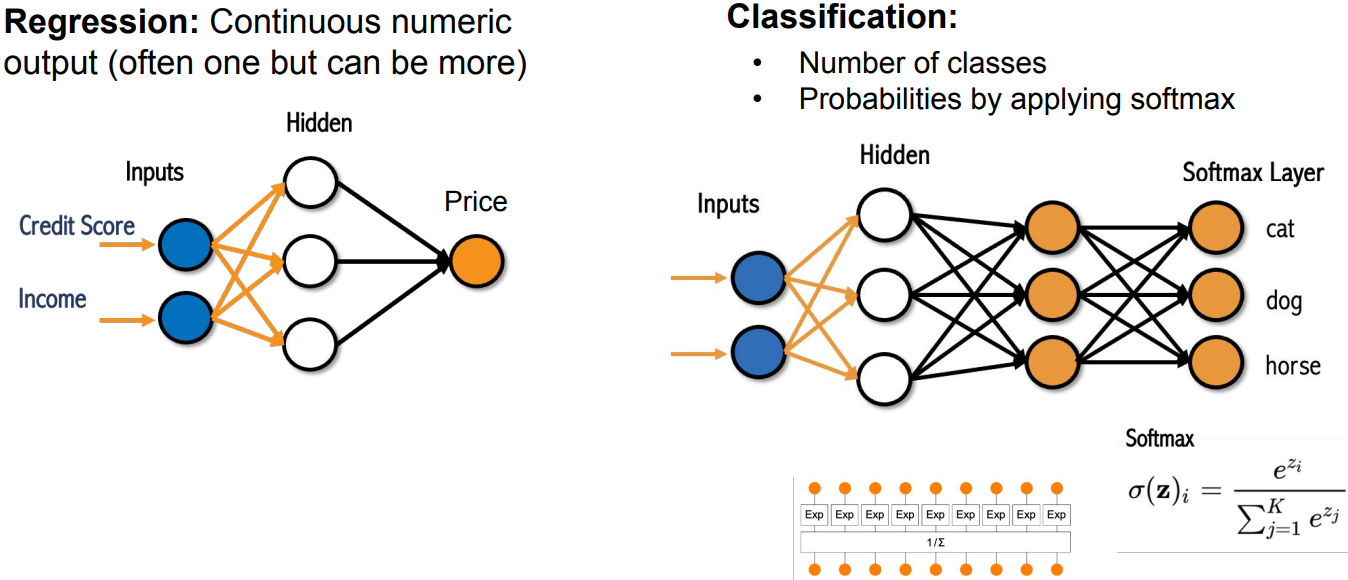
\includegraphics[width = \columnwidth]{figures/05/OutputNN.png}
\end{figure}
\subsubsection{Number of parameters}
Every connection(weights) + every Neuron(bias) = \# of parameters

	\section{Neural Networks}
Neural Networks are functions \(y = f(x,\theta)\) with parameters \(\theta\) that map mulitvariate inputs \(x\) to mulitvariate outputs \(y\).

\textbf{Unversal approximation theorem:} A shallow neural network (MLP) using nonlinear activation function can approximate any given continuous function defined ib a compact subset of \(R^D\) to arbitrary precision given enough hidden units (finite number).

\subsection{Loss function}
Regression: Mean squared error loss
\[
MSE = \frac{1}{N}\sum_{i=1}^{N}(y_i- \hat{y}_i)^2
\]
Classification: Cross entropy loss
\[
Loss = -\sum_{i= 1}^{\text{\#output classes}}y_i \cdot \log(\hat{y}_i)
\]
\subsection{Training}
Repeat:
\begin{itemize}
    \item Choose a training sample
    \item Forward pass: Compute the prediction
    \item Backward pass: If error > 0, update weights
\end{itemize}
Adjust weigths by Gradient descent
\[
w_i = w_i - \alpha\frac{\partial J(w_i)}{\partial w_i}
\]

Training Terms:
\begin{itemize}
    \item Epoch = a forward pass and backward pass complete for all the training examples
    \item Batch size = the number of training samples in a Batch
    \item Iteration = forward and backward pass each using a Batch
    \item Iterations per Epoch = \#training data /size of Batch
\end{itemize}
 Avoide overfitting with:
 \begin{itemize}
    \item Regularization (Lasso, Ridge)
    \item Dropout, turn off some neurons during training
    \item Batch normalization
    \item Early stopping
 \end{itemize}

 \subsection{Convolutional Neural Networks (CNN)}
 Idea: nearby pixels in an image are correlated - using shared parameters across whole input.
 A convolution operation is determined:
 \begin{itemize}
     \item stride (kernel shift)
     \item kernel size (typically odd)
     \item dilation (number of zero weights in kernel)
 \end{itemize}
 Convolutional Layer: apply convolution, add bias, apply activation function.

 Channels(feature maps, activation maps): mulitple convolutions applied to the input in parallel.
\subsubsection{CNN 1D}
\begin{figure}[!h]
    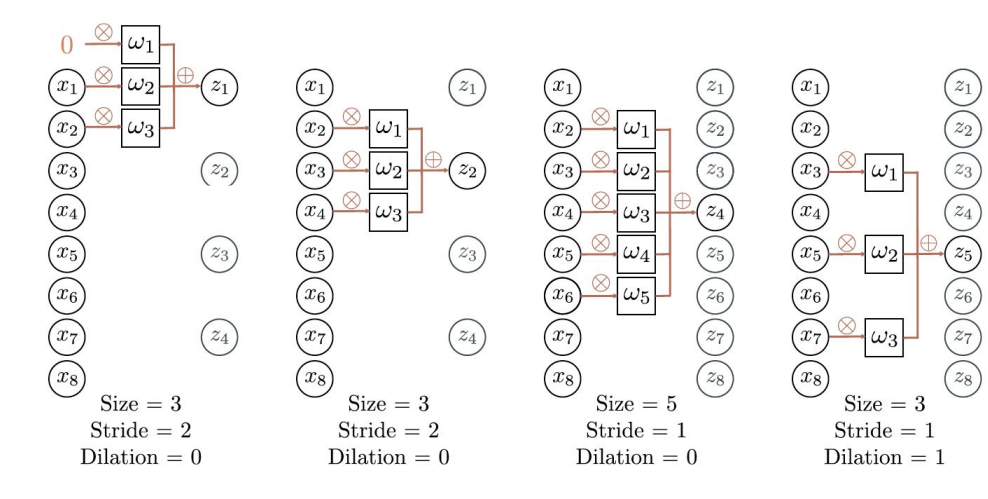
\includegraphics[width = \columnwidth]{figures/06/1DConv.png}
 \end{figure}
1D convolution is a weighted sum of nearby inputs.

\subsubsection{CNN 2D}
Using 2D kernles, plus a bias and a activation function.
\begin{figure}[!h]
    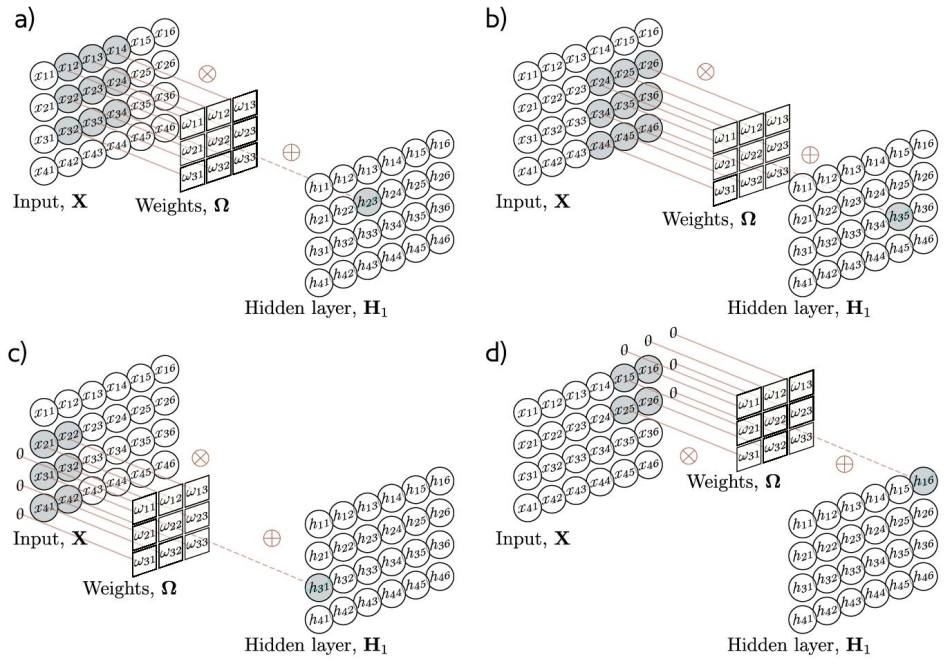
\includegraphics[width = \columnwidth]{figures/06/2DConv.png}
 \end{figure}

 \subsubsection{Pooling}
 Reduces Dimensions by min,max or average pooling a layer.
 \begin{figure}[!h]
    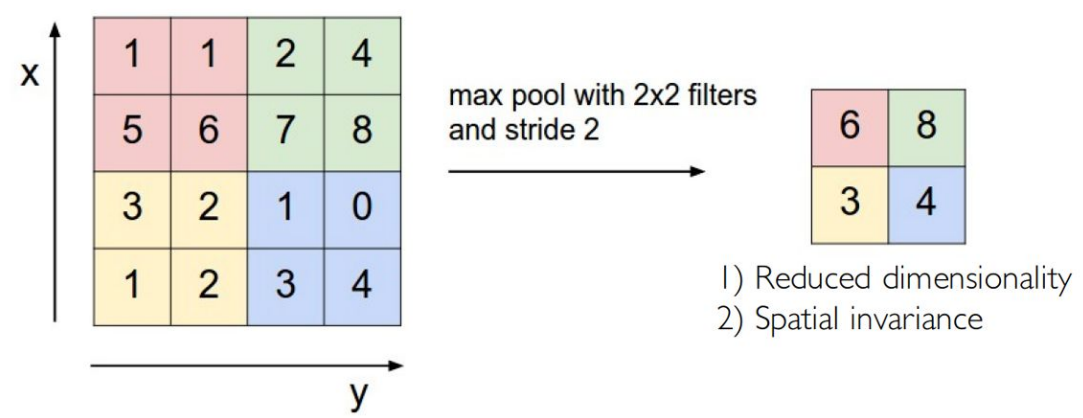
\includegraphics[width = \columnwidth]{figures/06/Pooling.png}
 \end{figure}
 \subsubsection{Transpose Convolution}
 Upsampling: Each input contributed multiple times to the output.
 Useful when output is an image.
	\section{Feature Engineering}
\subsection{Data Peparation and Exploration (EDA)}
Though exploratory data analysis (EDA) we can often:
\begin{itemize}
    \item discover important anomalies
    \item identify limitations in the collection process
    \item and better inform subsequent goal oriented analysis
\end{itemize}
Perpare, analyze and visualize data by unsing:
\begin{itemize}
    \item Histogramm, QQ-Plot
    \item Scatter-Matrix
    \item countplots, contingency tables
    \item Heatmaps
\end{itemize}

\subsection{Feature Preparation/generation}
\begin{itemize}
    \item Data \textbf{Cleaning}: Homogenize missing values and different types of the same feature, fix input errors, types, etc.
    \item \textbf{Aggregation|Pivoting}: Necessary when the entity to model is an aggregation from the provided data.
    \item \textbf{Imputation }of missing values. Strategies: mean, median, mode, using a model
    \item \textbf{Binarization}: Transform discrete or continuous numeric features into binary features
    \item \textbf{Binning} (fixed width, adaptive quantile binning): Split numerical values into bins and encode with a bin ID 
    \item \textbf{Transformation}(eg. Log-Transform, BoxCox): Compress the range of large numbers or expand the range of small numbers.
    \item \textbf{Scaling} and \textbf{normalizing} (min/max,z-score): Scale numerical variables into a certain range.
    \item \textbf{Generate Interaction features }
\end{itemize}
\subsection{Feature selection}
There are general two reasons why feature selection is used:
\begin{enumerate}
    \item Reducing the number of features, to reduce overfitting and improve the generalization of models
    \item To gain a better understanding of the features and their relationship to the response variables
\end{enumerate}
These two goals are often ar odds with each other.
\subsubsection{Univariate Feature Selection}
\begin{itemize}
    \item Based on univariate statistical tests.Examined for each feature individually
    \item Good for gaining a better understanding
    \item For regression: f\_regression, mutual\_info\_regression
    \item For classification: chi2, f\_classif, mutual\_info\_classif
\end{itemize}
Pearson Correlation Coefficient:
\[
\rho_{X_i,y} = \frac{\text{cov}[X_i,Y]}{\sigma_{X_i}\cdot \sigma_Y} = \frac{\mathbb{E}[X_i-\overline{X}_i]\cdot \mathbb{E}[Y-\overline{Y}]}{\sigma_{X_i}\cdot \sigma_Y}
\]
F-Regression test:
\[
\frac{\text{TSS}-\text{RSS}/p}{\text{RSS}/(n-p-1)} \sim F_{p,n-p-1}
\]
Mutual Information coefficant:
\[
I(X,Y) = \sum_{y \in Y} \sum_{x \in X} p(x,y)\cdot \log\left(\frac{p(x,y)}{p(x)\cdot p(y)}\right)
\]
\subsubsection{Feature selection using linear models \& regularization}
\begin{itemize}
    \item Lasso feature selection
    \item Ridge feature selection
    \item Linear Models: Subset selection
    \item Tree-based methods
\end{itemize}
\subsubsection*{Ridge feature selection}
Forces the coefficient values to be spread out more equally.
More usefull for feature interpertation then Lasso feature selection.

\subsubsection*{Linear Models}
Forward stepwise selection:
Let \(\mathcal{M}_0\) denote the null model with no predictors.
\begin{itemize}
    \item For \(k = 0,\dots,p-1\):
    \begin{enumerate}
        \item Consider all \((p-k)\) models that augment the perdictors in \(\mathcal{M}_k\) with one additional predictor.
        \item Choose the best among these \((p-k)\) models and call it \(\mathcal{M}_{k + 1}\). Here best is defined as having smallest \(RSS\) or highest \(R^2\).
    \end{enumerate}
    \item Select a single best model among \(\{\mathcal{M}_{0},\mathcal{M}_{1},\dots,\mathcal{M}_{p}\}\) using AIC or BIX or the adjusted \(R^2\)-score.
\end{itemize}
\subsubsection*{Metrics}
RSS = Residual Sum of Squares
\[
RSS = \sum_{i = 1}^{n}(y_i-\hat{y}_i)^2
\]
TSS 0 Total Sum of Squares
\[
    TSS = \sum_{i = 1}^{n}(y_i-\overline{y})^2
\]
\(R^2\)-score:(\% explained variance)
\[
R^2 = 1- \frac{RSS}{TSS}
\]
Adjusted \(R^2\)-score
\[
R^2_{adj} = R^2 = 1- \frac{\frac{RSS}{n-p-1}}{\frac{TSS}{n-1}}
\]
AIC(Akaike) and BIC(Bayesian) Information Criteria, \(\mathcal{L}\): Likelihood
\[
AIC = -2\log(\mathcal{L}) + 2p \qquad BIC = -2\log(\mathcal{L}) + 2\log(n) \cdot p
\]

\subsection{Text data/Natural Lannguage Processing (NLP)}
Text analysis is a major application field for ML algorithms.
To feed text to a algorithms it first has to be transformd to a numerical vector by:
\begin{itemize}
    \item \textbf{Tokenizing:} strings and give an integer ID to each possible token
    \item \textbf{Counting:} the occurences of token in each documnet
    \item \textbf{Normalizing:} and weighting with diminishing importance tokens that occur in the majority of samples/documents
\end{itemize}
\subsubsection{Tokenization}
\begin{enumerate}
    \item All common seperators, operators, punctuations and non-printable characters are removed(using Regex).
    \item Then, stop-words filtering that aims to filter-out the most frequent words performed
    \item Finally, stemming and/or lemmatization is applied to obtain the stem of a word that is morphological root by removing the suffixes that present grammatical or lexical infromation about the word.
\end{enumerate}
\textbf{Porter Stemming:} Simple replacement rules to create word roots.

\textbf{Lemmatization:} seeks to find actual roots for words.(e.g., tome \(\rightarrow\) book)
\subsubsection{Word Embeddings}
Idea: Map one-hot encoding to dense vectors
\begin{itemize}
    \item Each word is represented using a low-dimensional, dense, real-valued vector that encodes the meaning of the word such that the words that are closer in the vector space are expected to be similar in meaning
    \item How to compute them? Can be pre-trained using a very general task on a very large corpus or learnt with the target task
\end{itemize}
\begin{figure}
    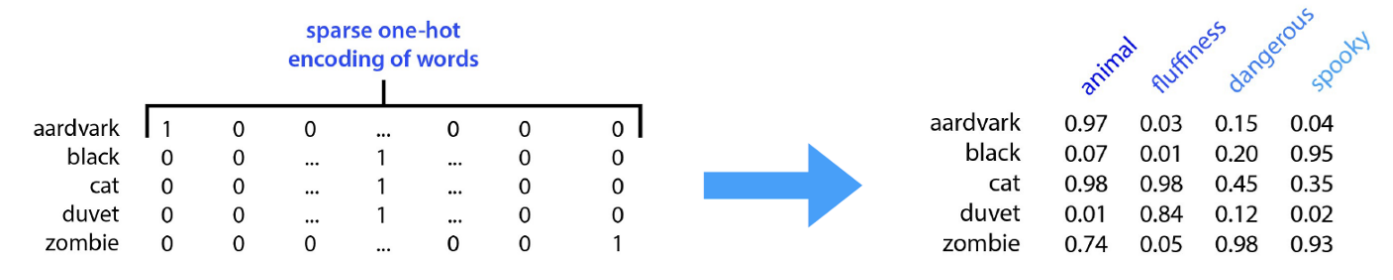
\includegraphics[width = \columnwidth]{figures/07/TextEmbeddings.png}
\end{figure}
This is called Word to vector(Word2Vec).
There are 2 variants:
\begin{itemize}
    \item continuous bad of words(CBOW)
    \item Skip-Gram
\end{itemize}
\subsection{Audio data}
In the time domain the resulting amplitudes, time delays (echos) are captured.
The fourier transform enables to decompose a signal into its individual frequencies an their amplitudes and phases.
\subsubsection{Linear predictive coding coefficients (LPC)}
LPC are parameters derived from audio signals that effectively model the spectral envelope of a sound wave.
They capture the articulatory constraints of the vocal tract.
\subsubsection{Spectogramm - Short Time Fourier Transform}
In many cases we have non periodic signals: frequency content varies over time. Compute FFT on overlapping windowed segments of the signal to obtain the spectogramm.
\begin{figure}[!h]
    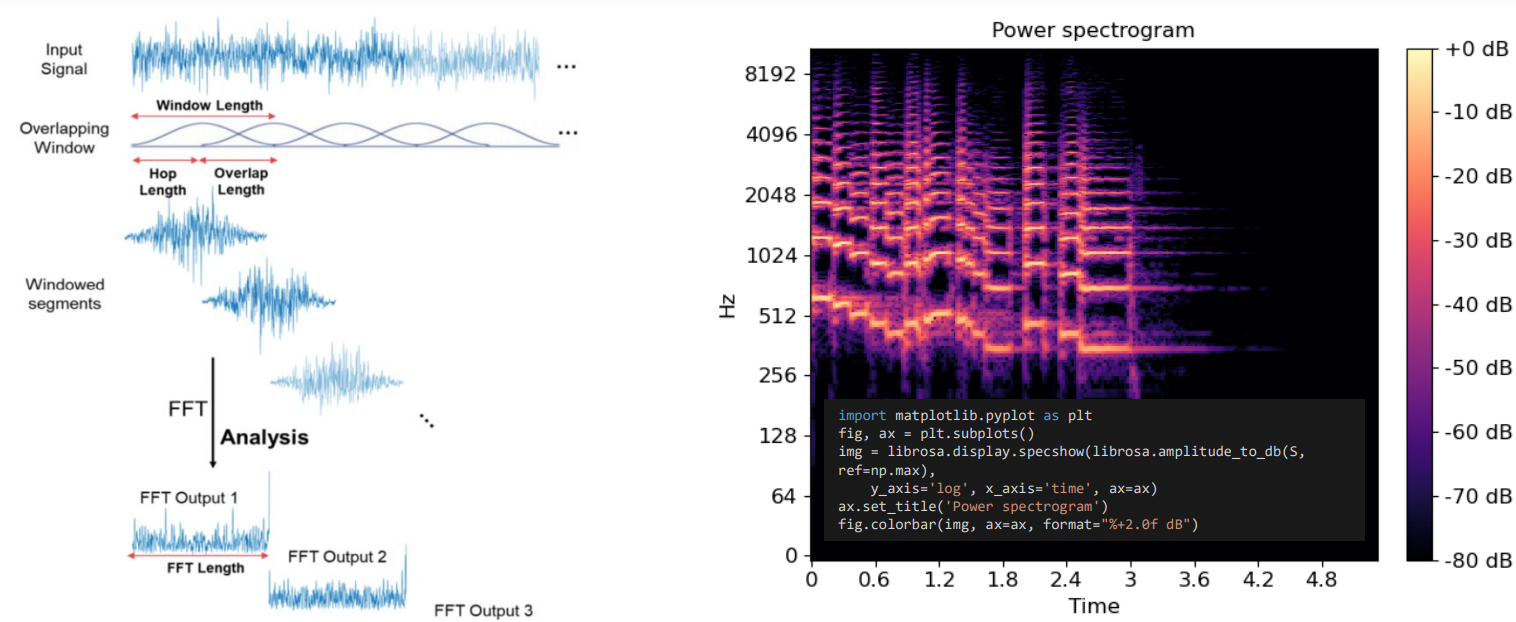
\includegraphics[width = \columnwidth]{figures/07/STFT.png}
\end{figure}
\subsubsection{Mel Frequency Cepstral Coefficients (MFCC)}
MFCC trys to mimic human hearing.
It condeses audio information into fewer coefficients, simplifying data without losing critical information.
They are noise robuster than raw spectral features.
\begin{figure}[!h]
    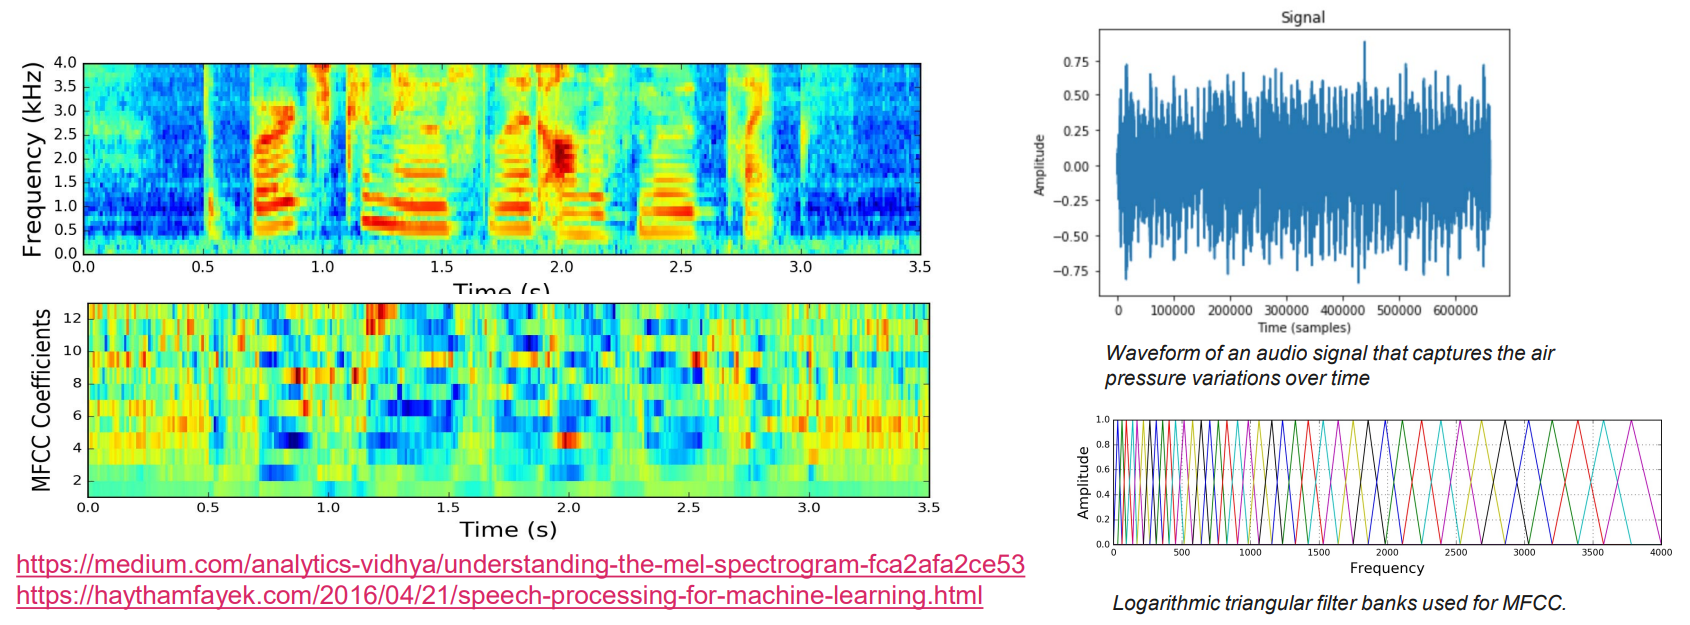
\includegraphics[width = \columnwidth]{figures/07/MFCC.png}
\end{figure}
	\section{Support Vector Machines}
	\section{Gaussian Processes}
\subsection{The Bayes optimal classifier}
Theoretically optimal (= most probable) classification.
Combine predictions of all hypotheses, weighted by their posterior probabilities: (where \(y_i\) is  a label from the set \(Y\) of classes)
\[
P(Y = y_k|X_1,\dots,X_n) = \frac{P(Y = y_k)\prod_{i} P(X_i|Y = y_k)}{\sum_j P(Y = y_j) \prod_i P(X_i|Y = y_j)}
\]
Naive Bayes Classifier:
\[
Y \leftarrow\arg\max_{y_k} P(Y = y_k)\prod_i P(X_i|Y = y_k)
\]
\subsection{Gaussian Distribution (1D)}
Norma distribution with mean \(\mu\) and variance \(\sigma^2\):
\[
p(x) = \mathcal{N}(x|\mu,\sigma^2) = \frac{1}{(2\pi\sigma^2)^{1/2}}\exp\left\{-\frac{1}{2\sigma^2}(x-\mu)^2\right\}
\]
\[
\mathbb{E}\left[x\right] = \mathbb{E}_{x \sim p}\left[x\right] = \int x\cdot p(x)\,dx = \mu
\]
\[
    \mathbb{E}\left[x^2\right] = \mathbb{E}_{x \sim p}\left[x^2\right] = \int x^2\cdot p(x)\,dx = \mu^2 + \sigma^2
\]
\[
\textbf{VAR}\left[x\right] = \mathbb{E}\left[x^2\right]-\mathbb{E}\left[x\right]^2 = \sigma^2
\]
\subsubsection{Mulitvariante Gaussian Distribution}
Gaussian defined over a vector \(x\) of continuous variables in a \(D\)-dimensional space with mean vector \(\mu\) and covariance matrix \(\Sigma\), where \(|\Sigma|\) is the determinant of \(\Sigma\).
\[
    p(\mathbf{x}) = \mathcal{N}(\mathbf{x} | \mu, \Sigma) = \frac{1}{(2\pi)^{D/2} |\Sigma|^{1/2}} \exp\left\{-\frac{1}{2} (\mathbf{x} - \mu)^T \Sigma^{-1} (\mathbf{x} - \mu)\right\}
\]
The quadratic form in the argument of the exponential is called \textbf{Mahalanobis distance}:
\[
\Delta = (\mathbf{x} - \mu)^T \Sigma^{-1} (\mathbf{x} - \mu)
\]
\subsection{Gaussian Processes}
A Gaussian process \(\mathcal{GP}\) is a stochastic process, i.e. a collection of random variables that are drawn from a infinite dimensional multivariate Gaussian distribution.
A stochastic process is a collection of random variables, \(\left\{h(x):x\in \mathcal{X}\right\}\) indexed by elements from some set \(\mathcal{X}\), known as the index set.
\subsubsection{Definition of a Gaussian Process\(\mathcal{GP}\)}
A Gaussian process is a stochastic process such that any finite subcollection of random variables has a multivariate Gaussian distribution(mean function \(m(\cdot)\) and convariance function \(k(\cdot,\cdot)\))
\[
\begin{bmatrix}
h(x_1) \\
\vdots \\
h(x_m)
\end{bmatrix}
\sim \mathcal{N} \left(
\begin{bmatrix}
m(x_1) \\
\vdots \\
m(x_m)
\end{bmatrix},
\begin{bmatrix}
k(x_1, x_1) & \cdots & k(x_1, x_m) \\
\vdots & \ddots & \vdots \\
k(x_m, x_1) & \cdots & k(x_m, x_m)
\end{bmatrix}
\right)
\]
 
\subsubsection{Example}
One dimensional Gaussian process:
\[
p(f(x))\sim \mathcal{GP}\left\{m(x) = 0,k(x,x') = \exp\left(-\frac{1}{2}(x-x')^2\right)\right\}
\]
To get an indication of what this distribution over functions looks like, focus on a finite subset of function values \(\textbf{f} = (f(x_1),f(x_2),\dots,f(x_n))\) for which:
\[
    \textbf{f} \sim \mathcal{N}(0,\Sigma)
\]
\[
\Sigma_{ij} = k(x_i,x_j)
\]
Then plot the coordinates of \textbf{f} as a function of the rorresponfing \(x\) values
\begin{figure}[!h]
    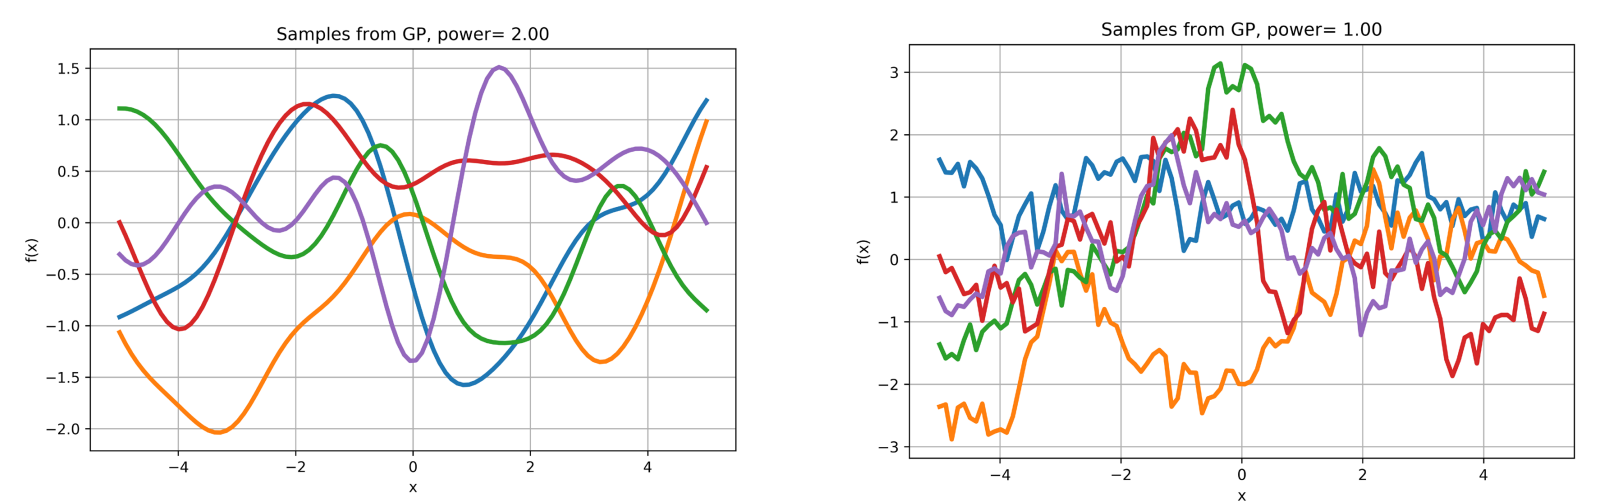
\includegraphics[width = \columnwidth]{figures/09/GPExample.png}
\end{figure}
\subsection{Covariance Function\(k(x,x') = \)Merver kernel}
Gaussian processes are kernel-based probability distribution in the sense that any valid kernel function can be used as a covariance function.
\(k(x,x')\) is a kernel, if there is a feature mapping \(\phi(x)\) into some (higher dimensional) space \(\mathcal{H}\), where it can be represented by a scalar (dot) product.

Some possible Kernels:
\begin{itemize}
    \item Radial Basis Function kernel (RBF)
    \[
    k(x,x') = \sigma_0^2\exp\left[-\frac{1}{2}(\frac{x-x'}{\lambda})^2\right]
    \]
    \item Rational-Quadratic kernel
    \[
    k(x,x') = \left(1 + \frac{(x-x')^2}{2\alpha\lambda^2}\right)^{-\alpha}
    \]
    \item Exp-Sine-Squared kernel
    \[
    k(x,x') = \exp\left[-\frac{2 \cdot \sin^2(\pi/p \cdot |x-x'|)}{\lambda^2}\right]
    \]
    \item Dot-Product kernel
    \[
    k(x,x') = \sigma^2_0 + x\cdot x'
    \]
\end{itemize}
	\section{Dimensionality Reduction}
\subsection{The Curse of Dimensionality}
One of the characteristic of high-dimensional data is that the number of dimensions is comparable or larger than the number of samples.
High dimensional data is very sparse
\begin{table}[!h]
    \begin{tabular}{l|l}
        \hline
     Dim \(d\)& \(n\) for 10\% coverage \\
     \hline
     1&  10\\
     2&  100\\
     3&  1000\\
     10& \(10^10\)\\
     d& \(10^d\)
    \end{tabular}
    \end{table}
\subsection{The Manifold Hypothesis}
A collection of methodologies for analyzing high dimensional data based on the hypothesis that data tend to lie near a low dimensional manifold is now called Mainfold learning.
\subsection{Principal Component Analysis (PCA)}
The main linear technique for dimensionality reduction, mapping the data in such a way that the variance of the data in the low-dimensional representation is maximized.
\subsubsection{Eigenvalues \(\lambda_k\) of \(
C\) are the variance in the new space}
We are given \(i = 1 \dots n\) samples of dimension\((1 \times d)\)
We constuct the data matrix \(n\times d\): \(X_{ik} = \left[x_{ik}\right]\)

We diagonalize the covariance matrix \(C\):
\[
C = \frac{1}{n-1}(X-\overline{X})^T (X-\overline{X})
\]
if \(\overline{X} = 0\):
\[
C = \frac{1}{n-1}X^T X
\]
\[
C = UDU^T = U\left[\text{diag}(\lambda_k)\right]U^T
\]
\subsubsection{Explained variance}
No data is lost in transformation.
The first component explains most of the variance, the second the second most,\dots All components explain the whole variance.
Now take only a few components (the first \(k\)) and hope that the data is explained by them.
How good is the approximation?
A measure is the \textbf{explained variance ratio}:
\[
P_k = \frac{\sum_{j = 1}^k\textbf{VAR}(Z:,j)}{\sum_{j = 1}^d\textbf{VAR}(Z:,j)} = \frac{\sum_{j = 1}^k\lambda_j}{\sum_{j = 1}^d\lambda_j} 
\]
\subsubsection{Eigenvalue problem}
\[
\mathbf{CW}-\lambda\mathbf{w} = 0
\]
\[
(\mathbf{C}-\lambda\cdot\mathbf{I})\mathbf{w} = 0
\]
\[
\det(\mathbf{C}-\lambda\mathbf{I}) = 0
\]
\subsection{Mainfold Methods based on similarity}
\subsubsection{Example of metrics}
\(L_p\) metric: \(d_p(x,y) = ||x-y||_p = \sqrt[p]{\sum_i|x_i-y_i|^p}\)

\(L_\infty\) metric: \(||x||_\infty = \max_i\left\{|x_i|\right\}\)

\(L_1\) metric: \(d_1(x,y) = ||x-y||_1 = \sum_i|x_i-y_i\) (manhatten distance)

\subsubsection{MDS: Multidimensional scaling}
MDS attemps to model similarity or dissimilarity data as distance in geometric spaces.
In general, is a technique used for analyzing similarity or dissimilarity data.
MDS attemps to find an embedding from the high dimensional objects in \(I\) into \(y_i \in \mathbb{R}^d\) such that distances \(d_{ij}\) are preserved.
\subsubsection{LLE: local linear embedding}
LLE discribes the local properties of the manifold around a data point \(x_i\) by writing the data point as a linear combination (the so-called reconstruction weights \(w_{ij}\)) of its \(k\) nearest neighbor:
\[
x_i \approx \sum_{j = 1}^k w_{ij}x_j
\]
In the low dimension, LLE attemps to retain the reconstruction weights \(W\) as well as possible. Hence, LLE fits a hyperplane through the data point \(x_i\) and its nearest neighbors, thereby assuming that the mainfold is locally linear.
Finding the low \(d\)-dimensional data representation \(Y\) amounts to minimizing the cost function \(\mathcal{L}\):
\[
\mathcal{L}(w,Y) = \sum_{i = 1}^{N}||y_i - \sum_{j = 1}^{k}w_{ij}y_j||^2
\]
\begin{figure}[!h]
    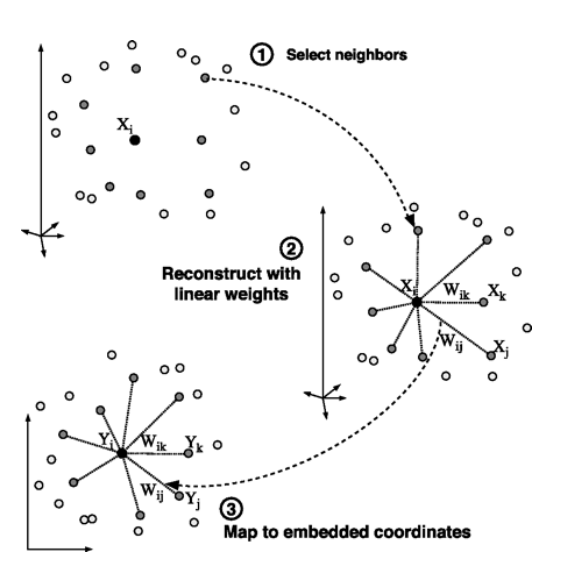
\includegraphics[width = \columnwidth]{figures/10/LLE.png}
\end{figure}
\subsubsection{Isomap: Isometric mapping}
A non-linear method for dimensionality reduction.
Finds the map that preserves the global, non-linear geometry of the data by preserving the geodesic manifold interpoint distances.
Geodesic: Shortest curve along the manifold connecting two points.
\begin{figure}[!h]
    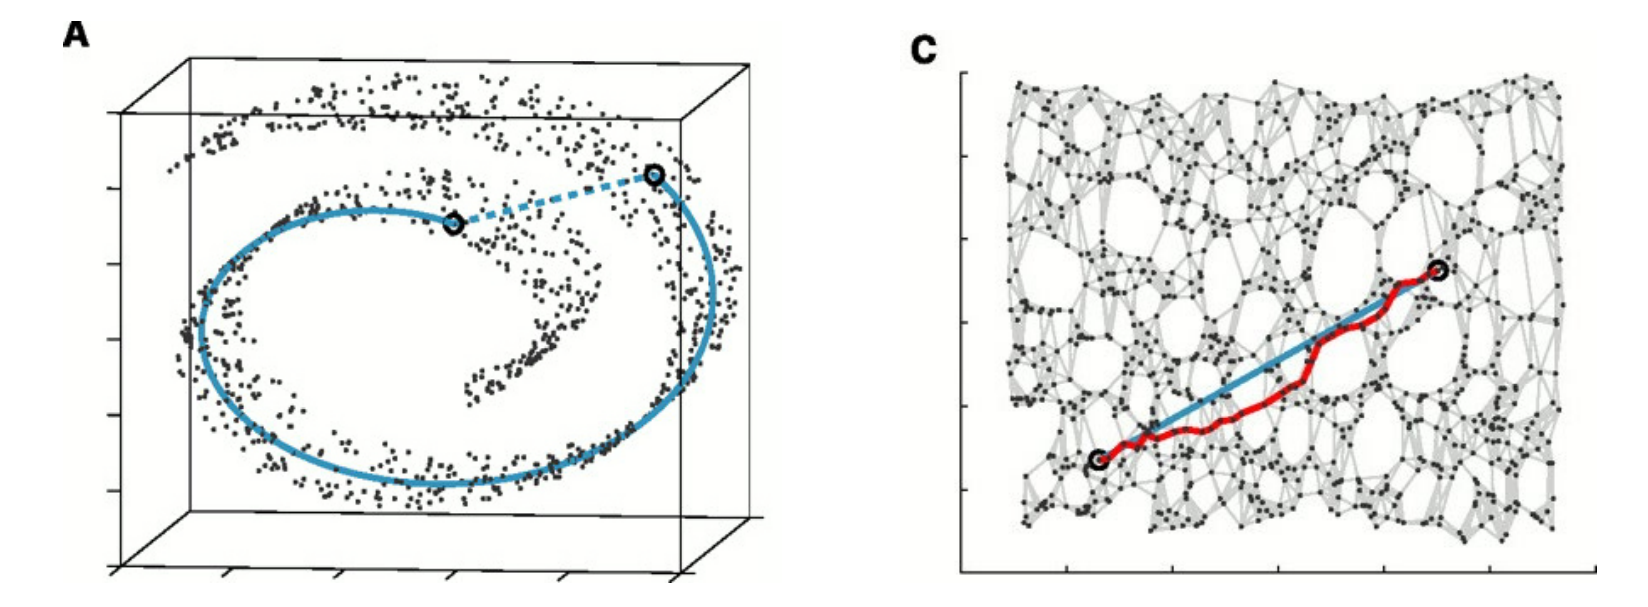
\includegraphics[width = \columnwidth]{figures/10/Isomap.png}
\end{figure}

The basic steps are:
\begin{enumerate}
    \item For each object, find a small set of neighboring objects and their distance.
    \item Compute all-pairs shortest paths on the above neighborhood graph.
    \item Run multidimensional scaling using the matrix of shortest-path distances.
\end{enumerate}
Advantages:
\begin{itemize}
    \item Nonlinear
    \item Non-iterative
    \item Globally optimal
    \item Parameters: \(k\) or \(\eta\)(chosen fixed radius)
\end{itemize}
Disadvantages:
\begin{itemize}
    \item Graph disctreteness overestimates the geodesic distance
    \item  \(k\) must be high to avoid linear shortcuts near regions of high surface curvature
\end{itemize}
\subsubsection{t-SNE:t-distributed stochastic neighbor embedding}
t-SNE is a manifold learning algorithem that constructs a probability distribution \(p\) over the dataset \(X\), and then another probability distribution \(q\) in a lower dimensional data space \(Y\), making both as close as possible

Baisc Steps:
\begin{enumerate}
    \item In the high dimensional space \(X\), create a probability distribution \(p_{i|j}\) that dictates the relationships between various neighboring points \(x_i\) and \(x_j\).
    \item It then tries to recreate a probability distribution \(q_{i|j}\) in a low dimensional space \(Y\) that follows that probability distribution \(p_{i|j}\) as best as possible (KL-divergence as loss function).
\end{enumerate}

\subsubsection*{Math}
\[
p_{i|j} = \frac{\exp\left(-\frac{||x_i-x_j||^2}{2\sigma_i^2}\right)}{\sum_{k\neq i}\exp\left(-\frac{||x_i-x_k||^2}{2\sigma_i^2}\right)}
\]
\[
q_{i|j} = \frac{e^{-||y_i-y_j||^2}}{\sum_{k\neq i}e^{-||y_i-y_k||^2}}
\]
The Kullback-Leibler (KL) divergence is a measure of how different two probability distributions are from one another (also called relative entropy):
\[
KL(P|Q) = \sum_{i \neq q}p_{i|j} \ln(\frac{p_{i|j}}{q_{i|j}})
\]
	\section{Cluster Analysis}

\begin{figure}[!h]
    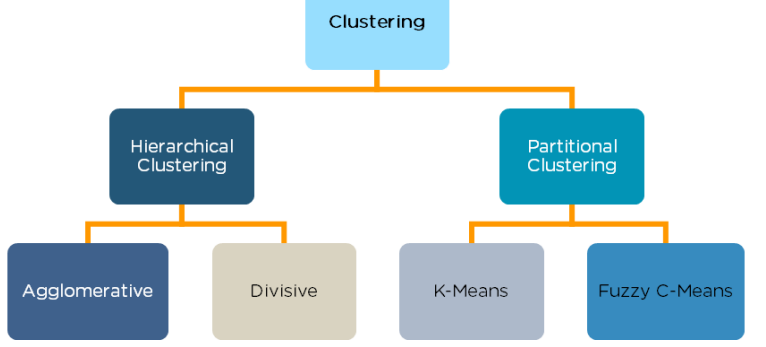
\includegraphics[width = \columnwidth]{figures/11/ClusteringOverview.png}   
\end{figure}
Clustering = Finding groups in data

Problem: given \(n\) data points, separate them into \(K\) clusters.
\begin{table}[!h]
    \begin{tabular}{ll}
    \(n\) &  number of data points\\
    \(K\) &  number of clusters \((K << n)\)\\
    \(\Delta\) &  a partition, \(\Delta = \{C_1,C_2,\dots,C_K\}\)\\
    \(\mathcal{L}(\Delta)\) & loss of \(\Delta\) to be minimized
    \end{tabular}
\end{table}

\subsection{Taxonomy of Clustering}
Hard clustering: Each data point is assigned a unique cluster:\(\Delta\)

Soft clustering: Each data point \(i\) is assigned a probability that it is in cluster \(k\):

Parametric clustering: \(k\) known

Non-parametric: \(k\) determined by algorithm
\subsection{Hierarchical Clustering}
Hierarchical Clustering (HCA) seeks to build a hierarchy of clusters.
Strategies for hierarchical clustering generally fall into two types:
\begin{itemize}
    \item Agglomerative: This is a bottom-up approach: each observation starts in its own cluster, and pairs of clusters are merged as one moves up their hierarchy.
    \item Divisive: This is a top-down approach: all observations start in one cluster, and splits are performed recursively as one moves down the hierarchy.
\end{itemize}
We start with \(N\) datapoints that initially form \(N\) clusters.
The two clusters with the smallest linkage are fused togther to form \(N - 1\) clusters.
This is repeated until there is only one single cluster.
\[
(i,j)_{fused} = \arg\min_{i \neq j}\{D_{link}(C_i,C_j)\}
\]
\subsubsection{Linkage criteria}
The linkage citerion determines together with a metric \(d(x,y)\) when two clusters \(A\) and \(B\) should be merged together in hierarchical clustering (fusion criterium)
\begin{table}[]
    \begin{tabular}{ll}
    Maximum(complete) &  \(\max\{d(a,b): a\in A,b\in B\}\)\\
    Minimum(single) &  \(\min\{d(a,b):a\in A,b\in B\}\)\\
    Mean(average) &  \(\frac{1}{|A|\cdot|B|}\sum_{a\in A}\sum_{b\in B}d(a,b)\)\\
    Centroid & \(||c_s-c_t||\)
    \end{tabular}
\end{table}

where \(c_s\) and \(c_t\) are the centroids of clusters \(s\) and \(t\), respectively.
\begin{figure}[!h]
    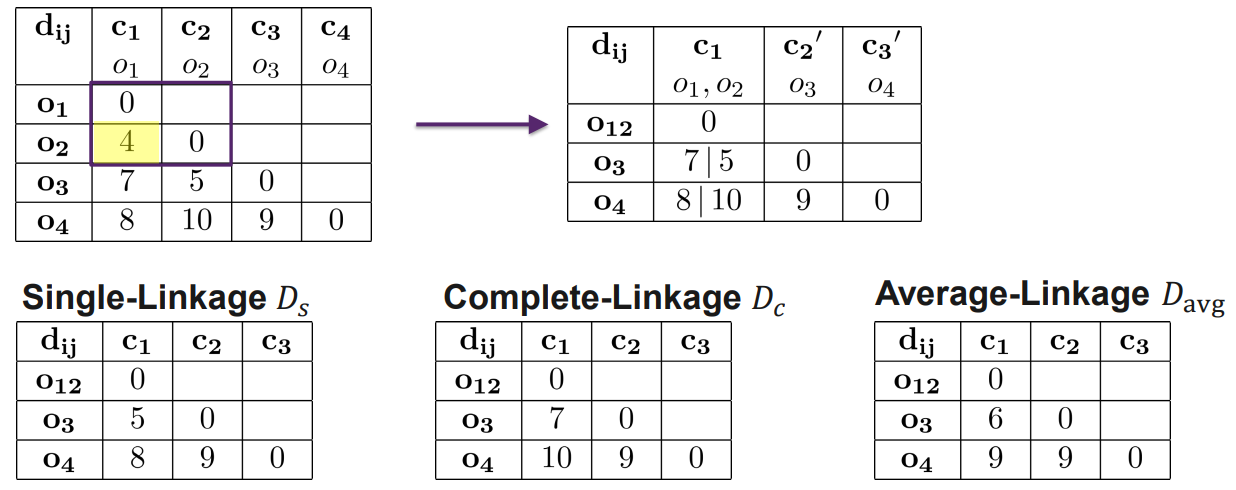
\includegraphics[width = \columnwidth]{figures/11/ExampleHCA.png}    
\end{figure}

\subsubsection{Basic Algorithm}
Input:
\begin{itemize}
    \item Distance matrix \(D\) data points (size \(n\times n\))
    \item fucntion \(d(a,b)\) to compute a distance between clusters (usually takes \(D\) as input)
\end{itemize}
Initialization: Clustering \(\mathcal{C}^{(0)} = \{C_1^{(0)},C_2^{(0)},\dots,C_n^{(0)}\} = \{i\}\)

While the current number of clusters is \(>1\):
\begin{itemize}
    \item find the two clusters which have the smallest linkage to each other
    \item merge them to one cluster
\end{itemize}
Ouput: Resulting Dendrogram: The Dendrogram is a tree that represent the hierarchical division of the data set \(O\) into ever smaller subsets.


Dendrograms cannot tell you how many clusters you should have: Interpretation of this kind is justified only when the ultrametric tree inequality holds, which is very rare.
\begin{figure}[!h]
    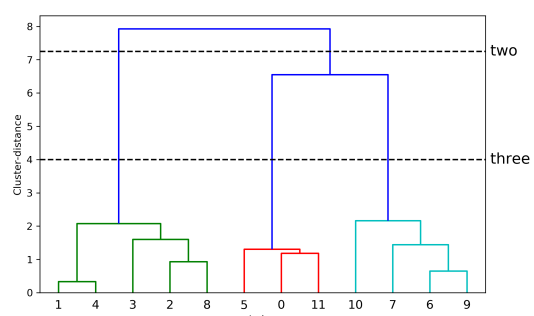
\includegraphics[width = \columnwidth]{figures/11/Dendrogram.png}
\end{figure}


\subsection{K-means}
\begin{figure}[!h]
    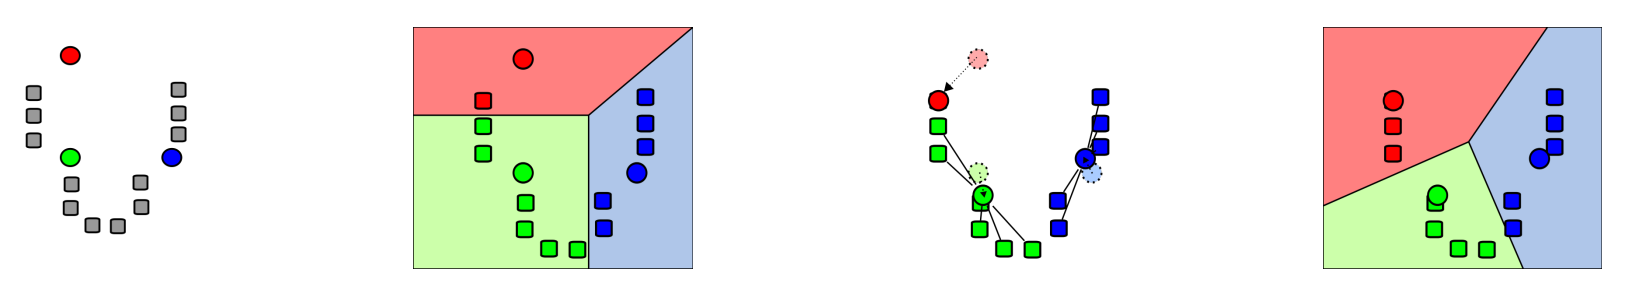
\includegraphics[width = \columnwidth]{figures/11/KMeansExample.png}
\end{figure}
The standard algorithem is non-probabilistic EM.
The problem is that k-means is very sensitive to the choice of \(k\), even with correct \(k\) it may converge to wrong local Minimum.
\subsubsection{K-means algorithm}
Input: Data \(\mathcal{D} = \{x_i\}_{i = 1:N}\), number of clusters \(K\)

Initialize: centers \(\mu_1,\mu_2,\dots,\mu_k \in \mathbb{R}^d\) at random

Iterate until convergence:
\begin{enumerate}
    \item for \(i = 1:n\): \(k(i) = \arg\min_k||x_i-\mu_i||\)(assign points to cluster \(\rightarrow\) new clustering)
    
    \item for \(k = 1:K\): \(\mu_k = \frac{1}{|C_k|}\sum_{i \in C_k}x_i\) (recalcuate centers)
\end{enumerate}
Convergence: if \(\Delta\) does not change after iteration \(m\), it will never change after that.

How to pick starting points?:
\begin{itemize}
    \item Random initialization: Randomly choose some data points as starting centers.
    \item Forgy method: Chooses \(k\) observations from the dataset and uses these as the initial means.
    \item Random Partition: Randomly assignes a cluster to each observation an then proceeds to the update step, thus computing the initial mean to be the centroid of the clusters randomly assigned points.
    \item K-means++: The algorithm is guaranteed to find a solution that is \(O(\log k)\) competitive to the optimal k-means solution.
\end{itemize}
\subsubsection{K-means cost function}
The distortion(least-squares) can also be expressed as sum of (squared) intracluster distances:
\[
\mathcal{L}(\Delta) = \frac{1}{2}\sum_{k = 1}^K\sum_{i\in C_k}||x_i - x_j||^2 + \text{const}
\]
\subsubsection{Limitations of K-means: Non-globular shapes}
\begin{enumerate}
    \item Inertia W makes the assumption that clusters are convex and isotropic.
    \item Inertia W is not a normalized metric.
\end{enumerate}
\subsubsection{More variants of K-means}
\begin{itemize}
    \item K-medians
    \item weighted K-means: weighted data points
    \item kernel-k-means
    \item soft K-means: soft assignments (in form of probability)
\end{itemize}

\subsubsection{How shall we choose \(k\)}
\begin{itemize}
    \item Basic Elbow method
    \item Try a range of \(K\) values and plot average distance to centers
    \item Silhoutte
    \item Cross-Validation
    \item Information theoretic perspective: NMI,BIC and AIC
\end{itemize}

\subsubsection*{Silhoutte Score}
A graphical method to select \(k\).
Given K and K clusters, given any data point \(i\), let \(a_i\) be the average distance or dissimilarity of \(i\) with all other points in the same cluster.
\(a_i\) measures how well \(i\) fits into its own cluster.
\(b_i\) is the smallest average distance(Euclidean distance) of \(i\) to other clusters.

Silhouette score \(s_i \in \left[-1,1\right]\):
\[
s_i = \frac{b_i - a_i}{\max(b_i,a_i)}
\]
\(s_i\approx 1\): point \(i\) is in a tight cluster and far away from other clusters

\(s_i\approx -1\): point \(i\) is in a loose cluster and close to other clusters

Maximize \(\frac{1}{n}\sum_{i = 1}^n s_i\) over \(k\).



	\section{Gaussian Mixture Models and EM}
	\section{Reinforcement Learning}
\begin{figure}[!h]
    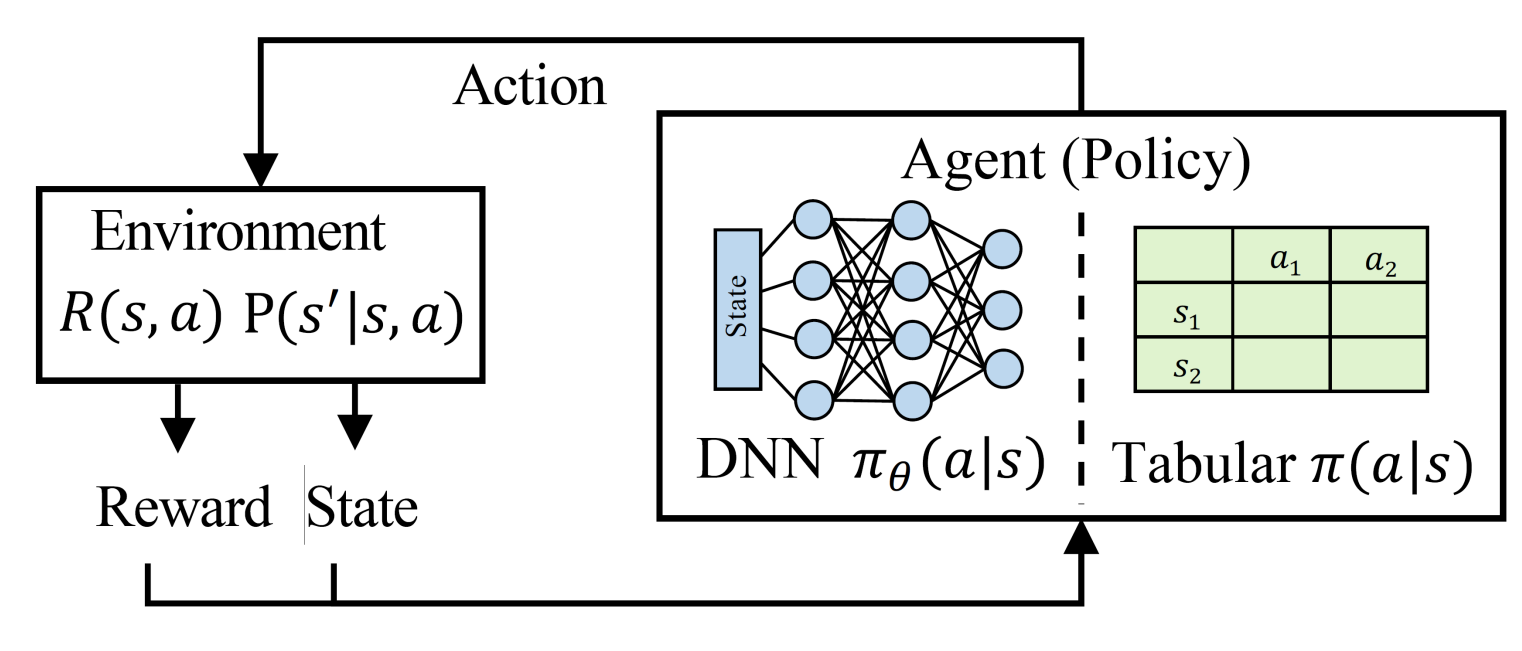
\includegraphics[width = \columnwidth]{figures/13/AgentEnvironment.png}    
\end{figure}
\begin{figure}
    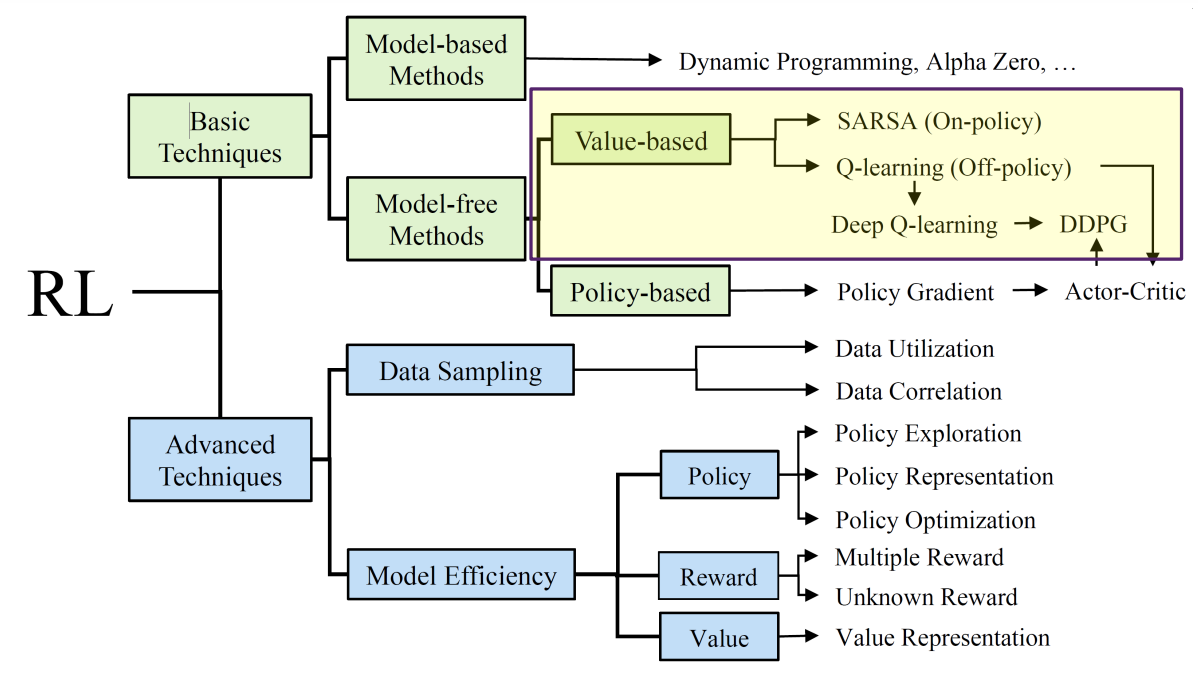
\includegraphics[width = \columnwidth]{figures/13/OverviewRL.png}
\end{figure}
The agent and environment interact at each of a sequence of discrete time steps,\(t = 0,1,2,\dots\).
At each time step \(t\), the agent receives some representation of the environment's states,\(s_i \in S\), where \(S\) is the set possible states.
On that basis, the agent selects an action, \(a\in A(s_t)\), where \(A(s_t)\) is the set of actions available in state \(s_t\).
One time step later, in part as a consequence of its action, the agent receives a numerical reward,\(R_{t+1}\in \mathbb{R}\), and finds itself in a new state, \(s_{t+1}\).
\subsubsection{Policy \(\pi\)}
A policy \(\pi\) is a distribution over actions \(a\) given state \(s\),i.e. it is the probability that the agent takes action \(a_t \in A\) in state \(s \in S\)
\[
\pi(a|s) = Pr\left[a_t = a|s_t = s\right]
\]
\subsubsection{Types of RL environments}
\begin{itemize}
    \item Deterministic environment
    \item Stochastic environment
    \item Fully observeable environment
    \item Partially observeable environment
    \item Discrete environment
    \item Continuous environment
    \item Episodic and non-episodic environment
    \item Single and multi-agent environment
\end{itemize}
\subsubsection{Agent Categories}
\begin{itemize}
    \item Value Based: No policy, Value function
    \item Policy Based: Policy, No value function
    \item Actor Critic: Policy(for the actor), Value function (for the critic)
    \item Model Free: Policy and/or Value function, no (explicit) Model of the Environment, no explicit dynamics Model
    \item Model Based: Optionally Policy and/or Value function, (explicit) Model of the Environment, explicit dynamics Model
\end{itemize}
\subsubsection{Markov Process}
A Markov Process (or Markov Chain) is a tuple (S,P), where:
\begin{itemize}
    \item \(S\) is a (finite) set of states
    \item \(P\) is a state transition probability matrix(Markov table): \(P_{ss'} = Pr(s_{t+1}|s_t)\)
\end{itemize}
The core concept is that the future only depends in the present and not on the past.
\subsubsection{Markov Reward Process (MRP)}
A Markov Reward Process is a tuple \((S,P,\mathcal{R},\gamma)\):
\begin{itemize}
    \item \(S\) is a (finite) set of states
    \item \(P\) is a state transition probability matrix:\(P = P_{ss'} = Pr(s_{t+1}|s_t)\)
    \item \(\mathcal{R}\) is a reward function (expectation value of the next reward): \(\mathcal{R}_s = \mathbb{E}\left[R_{t+1}|s_t\right]\)
    \item \(\gamma\) is a discount factor: \(\gamma \in \left[0,1\right]\)
\end{itemize}
\subsection{Markov decision process (MDP = MRP + A)}
A Markov Decision Process is a tuple \((S,A,P,\mathcal{R},\gamma)\)
\begin{itemize}
    \item \(S\) is a (finite) set of states
    \item \(A\) is a (finite) set of actions
    \item \(P\) is a state transition probability matrix:\(P = P_{ss'} = Pr(s_{t+1}|s_t)\)
    \item \(\mathcal{R}\) is a reward function (expectation value of the next reward): \(\mathcal{R}_s = \mathbb{E}\left[R_{t+1}|s_t\right]\)
    \item \(\gamma\) is a discount factor: \(\gamma \in \left[0,1\right]\)
\end{itemize}

\subsubsection{Return \(G_t\)}
The Return \(G_t\) is the total discounted reward from time-step \(t\) on.
\[
G_t = R_{t+1} + \gamma R_{t+2} + \dots = \sum_{k = 0}^{\infty} \gamma^k R_{t+k+1}
\]
\begin{itemize}
    \item \(\gamma\) close to 0 leads to myopic evaluation
    \item \(\gamma\) close to 1 leads to far-sighted evaluation
\end{itemize}
Recursion formula (basis for the Bellman equation):
\[
G_t = R_{t+1} + \gamma G_{t+1}
\]
\subsubsection{Value Function \(V(s)\) and Bellman Equation for MRP}
The state-value-function \(V(s)\) of an MRP is the expected cumulated return starting from state \(s\);
\[
V(s) = \mathbb{E}\left[G_t|s_t = s\right]
\]
The state-value-function can be decomposed in two parts.
This leads to the Bellman Equation for MRPs
\[
V(s) = \mathcal{R}_s + \gamma \sum_{s'\in S}P_{ss'}V(s') 
\]
Bellman's principle of optimality: in many mathematical optimitzation problems, the optimum (global) solution is a sequence of optimum partial solutions.

\subsubsection{State-action-value funtion \(Q(s,a)\)}
The state-action-value function \(Q(s,a)\) is a expected return starting from state \(s\), taking action \(a\), and then following policy \(\pi\).
It can be decomposed:
\begin{align*}
    Q^\pi(s,a) &= \mathbb{E}_\pi\left[G_t|s,a\right]\\
    &= \mathbb{E}_\pi\left[R_{t+1} + \gamma Q^\pi(s_{t+1},a_{t+1})|s,a\right]
\end{align*}

The Bellmen Equation for \(Q^\pi(s,a)\):
\[
Q^\pi(a,s) = \mathcal{R}_s^a + \gamma \sum_{s'\in S}P^a_{ss'}\sum_{a' \in A}\pi(a'|s')\cdot Q^\pi(s',a')
\]
\subsubsection{Maximum value function: max.expected future reward}
Goal of the MDP: the optimum policy
\[
V^*(s) = \max_{\pi}\left\{V^\pi(s)\right\}
\]
\[
Q^*(s,a) = \max_{\pi}\left\{Q^\pi(s,a)\right\}
\]
\subsection{Temporal-Difference (TD) Learning}
There are two concepts for solving Markov decision processes (MDPs).
\begin{itemize}
    \item Monte Carlo(MC) techiques
    \item Dynamic Programming(DP)
\end{itemize}
Temporal-difference (TD) learning is a combination of these two approaches. 
It learns directly from experience by sampling, but also bootstraps.
This represents a breakthrough in capability that allows agents to learn optimal strategies in any environment.
\subsubsection{Updating the Value Function}
\textbf{Monte Carlo:} The value function \(V(s)\) is updated by averaging the returns observed from multiple episodes that pass through state \(s\), where \(G_t\) is the return (cumulative discounted reward) following state \(s\) at time \(t\) and \(\alpha\) is the learning rate.
\[
V^{(t+1)}(s) = V^{(t)}(s) + \alpha\left[G_t - V^{(t)}(s)\right]
\]

\textbf{Bootstrapping methods}, such as those used in Temporal-Difference (TD) learning, update the value function based on estimates rather than waiting for the final outcome.
These methods can update the value function after each time step, leading to faster learning.

Bootstrapping TD-Learning:
\[
V^{(t+1)}(s) = V^{(t)}(s) + \alpha\left[r + \gamma V^{(t)}(s') - V^{(t)}(s)\right]
\]

Temporal-difference state-value function:
\[
V_\pi(s) = \mathbb{E}\left[V_\pi(s) + \alpha(r + \gamma V_\pi(s')-V_pi(s))|s\right]
\]

Online TD state-value estimate:
\[
V_\pi(s) \leftarrow V_\pi(s) + \alpha\left[r + \gamma V_\pi(s')\right] = V_\pi(s) + \alpha \left[V_{target} - V_\pi(s)\right]
\]


	% \section{Generative AI}

\end{document}
